\documentclass[final]{article}


\usepackage[nonatbib]{neurips_2024}

% ------------------------------------------------------------
%  2) Explicitly load natbib with numeric style:
% ------------------------------------------------------------
\usepackage[numbers,sort&compress]{natbib}

% ------------------------------------------------------------
% 3) Choose a numeric bibliography style for consistency:
%    (abbrvnat, unsrtnat, plainnat, etc. all work with natbib)
%    We'll set this at the end with \bibliographystyle{abbrvnat}.
% ------------------------------------------------------------

% ------------------------------------------------------------
% 4) Standard math & other packages (remove duplicates):
% ------------------------------------------------------------
\usepackage{amsmath,amssymb,amsfonts,amsthm}
\usepackage{colortbl}
\usepackage{algorithm}
\usepackage{algpseudocode}
\usepackage{arydshln}
\usepackage{graphicx}
\usepackage{multirow}
\usepackage{textcomp}
\usepackage{pgfplots}
\usepackage{xcolor}
\usepackage{dsfont}
\usepackage[utf8]{inputenc} 
\usepackage[T1]{fontenc}
\usepackage{url}
\usepackage{booktabs}
\usepackage{nicefrac}
\usepackage{microtype}
\usepackage{tabularx}
\usepackage{array}
\usepackage{hyperref}


\newcolumntype{C}[1]{>{\centering\arraybackslash}p{#1}}
\newcommand{\mn}[1]{\textcolor{blue}{X: #1}}
\newcommand{\graytext}[1]{\textcolor{gray}{\scriptsize #1}}
\newcommand{\ms}[1]{\textcolor{red}{Mohammad: #1}}
\newcommand{\bd}[1]{\textcolor{violet}{Bahar: #1}}
\newcommand{\ali}[1]{\textcolor{teal}{Ali: #1}}
\newcommand{\moein}[1]{\textcolor{purple}{Moein: #1}}
\newcommand{\kian}[1]{\textcolor{magenta}{Kian: #1}}

\newcommand{\theHalgorithm}{\arabic{algorithm}}

\DeclareMathOperator{\poly}{poly}
\DeclareMathOperator{\tr}{tr}
\DeclareMathOperator*{\argmin}{arg\,min}

\title{Scanning Trojaned Models Using Out-of-Distribution Samples}


% The \author macro works with any number of authors. There are two commands
% used to separate the names and addresses of multiple authors: \And and \AND.
%
% Using \And between authors leaves it to LaTeX to determine where to break the
% lines. Using \AND forces a line break at that point. So, if LaTeX puts 3 of 4
% authors names on the first line, and the last on the se  Detecting Backdoor Attacks on Deep Neural Networks by


%%%%%%%%%%%%%%%%%%%%%%%%%%%%%%%%
% THEOREMS
%%%%%%%%%%%%%%%%%%%%%%%%%%%%%%%%
\theoremstyle{plain}
\newtheorem{theorem}{Theorem}
\newtheorem{proposition}[theorem]{Proposition}
\newtheorem{lemma}[theorem]{Lemma}
\newtheorem{condition}[theorem]{Condition}
\newtheorem{corollary}[theorem]{Corollary}
\theoremstyle{definition}
\newtheorem{definition}[theorem]{Definition}
\newtheorem{assumption}[theorem]{Assumption}
\theoremstyle{remark}
\newtheorem{remark}{Remark}


\pgfplotsset{compat=1.18}

\begin{document}
\pdfoutput=1


% \author{%
% \small
%   Hossein Mirzaei \thanks{Department of Computer Engineering, Sharif University of Technology, Tehran, Iran} \\
%   \And
%   Ali Ansari \footnotemark[1] \thanks{Equal contribution.} \\
%   \And
%   Bahar Dibaei Nia \footnotemark[1] \footnotemark[2]\\
%   \And
%   Mojtaba Nafez \footnotemark[1] \thanks{Equal contribution.} \\
%   \And
%   Moein Madadi \footnotemark[1] \footnotemark[3]\\
%   \And
%   Sepehr Rezaee \footnotemark[1] \footnotemark[3]\\
%   \And
%   Zeinab Sadat Taghavi \footnotemark[1] \\
%   \And
%   Arad Maleki \footnotemark[1]\\
%   \And
%   Kian Shamsaie \footnotemark[1]\\
%   \And
%   Mahdi Hajialilue \footnotemark[1]\\
%   \And
%   Jafar Habibi \footnotemark[1]\\
%   \And
%   Mohammad Sabokrou 
%   % \thanks{Okinawa Institute of Science and Technology, Okinawa, Japan}
%   \\
%   \And
%   Mohammad Hossein Rohban \footnotemark[1]\\
% }
% 
\begingroup
   \renewcommand{\thefootnote}{}% temporarily clear the footnote symbol
   \footnotetext{For correspondence, please contact: <\texttt{rohban@sharif.edu}>,%
  \quad <\texttt{hossein.mirzaeisadeghlou@epfl.ch}>.}
\endgroup

\author{
Hossein Mirzaei$^{1}$ \quad Ali Ansari$^{2}$ \thanks{Equal Contribution} \quad Bahar Dibaei Nia$^{2}$ \footnotemark[1] \\ \\
\textbf{Mojtaba Nafez}$^2$ \thanks{Equal Contribution} \quad \textbf{Moein Madadi} $^2$ \footnotemark[2] \quad
\textbf{Sepehr Rezaee}$^3$ \footnotemark[2] \\ \\
\quad \textbf{Zeinab Sadat Taghavi}$^2$ \quad \textbf{Arad Maleki}$^2$ \quad \textbf{Kian Shamsaie}$^2$ \quad \textbf{Mahdi Hajialilue}$^2$ \\ \\ \quad \textbf{Jafar Habibi}$^2$ \quad \textbf{Mohammad Sabokrou}$^3$ \quad \textbf{ Mohammad Hossein Rohban}$^2$\\
\\
$^1$École Polytechnique Fédérale de Lausanne (EPFL) \quad $^2$Sharif University of Technology \\ \quad $^3$Shahid Beheshti University  \quad $^4$Okinawa Institute of Science and Technology\\
% \texttt{\{yangk,tianjunz,jegonzal,klein\}@berkeley.edu}\\
% \texttt{\{cummins,bcui,benoitsteiner,yuandongt\}@fb.com}\\
% \texttt{linnan\_wang@brown.edu}
}

\maketitle



\begin{abstract}
Scanning for trojan (backdoor) in deep neural networks is crucial due to their significant real-world applications. There has been an increasing focus on developing effective general trojan scanning methods across various trojan attacks. Despite advancements, there remains a shortage of methods that perform effectively without preconceived assumptions about the backdoor attack method. Additionally, we have observed that current methods struggle to identify classifiers trojaned using adversarial training. Motivated by these challenges, our study introduces a novel scanning method named \textbf{TRODO} (\textbf{TRO}jan scanning by \textbf{D}etection of adversarial shifts in \textbf{O}ut-of-distribution samples). TRODO leverages the concept of "blind spots"—regions where trojaned classifiers erroneously identify out-of-distribution (OOD) samples as in-distribution (ID). We scan for these blind spots by adversarially shifting OOD samples towards in-distribution. The increased likelihood of perturbed OOD samples being classified as ID serves as a signature for trojan detection. TRODO is both trojan and label mapping agnostic, effective even against adversarially trained trojaned classifiers. It is applicable even in scenarios where training data is absent, demonstrating high accuracy and adaptability across various scenarios and datasets, highlighting its potential as a robust trojan scanning strategy. The code repository is available at: \url{https://github.com/rohban-lab/TRODO}.
% Scanning trojaned deep learning models is a critical task due to their widespread real-world applications. Recently, there has been a growing focus on developing general trojan scanning methods that can perform effectively across various strategies used to trojanize input models. Despite advancements in proposed scanning methods, still there is a lack of a scanning method that performs effectively without any preassumptions about the input trojaned classifier. Moreover, we experimentally observe that existing scanning methods fall short in identifying trojaned classifiers that have been trojanized with adversarial training. Motivated by this, our study proposes a novel scanning method, TRODO (\textbf{TRO}janed scanning by \textbf{D}etection of Adversarial Shifts in \textbf{O}OD Samples), which leverages the concept of "blind spots"—regions where trojaned classifiers misclassify out-of-distribution (OOD) samples as in-distribution (ID). TRODO identifies these blind spots by adversarially perturbing OOD samples to shift them toward ID. The changes in the likelihood of perturbed OOD samples belonging to ID serve as a signature for trojan detection. TRODO is general, both trojan and target label agnostic, and effective even against adversarially trained trojaned classifiers. Extensive evaluations demonstrate TRODO's high accuracy and adaptability across various scenarios and datasets, highlighting its potential as a general trojan scanning strategy.
% Deep Neural Network (DNN)-based models are extensively utilized in critical applications such as image classification, face recognition, and autonomous driving. However, their reliability is increasingly challenged by trojan attacks, where adversaries introduce malicious samples into the training data, causing the model to perform normally on clean data but fail on trojaned samples. Existing defense strategies, such as trojaned model scanning, have limitations in their generality and effectiveness, particularly against adversarially trained models. This study proposes a novel scanning method, TRODO (TROjaned model scanning by Detection of Adversarial Shifts in OOD Samples), which leverages the concept of "blind spots"—regions where trojaned classifiers misclassify out-of-distribution (OOD) samples as in-distribution (ID). TRODO identifies these blind spots by adversarially perturbing OOD samples to mimic trojan triggers, significantly increasing their ID scores. This method is general, trojan and trigger agnostic, and effective even against adversarially trained classifiers. Extensive evaluations demonstrate TRODO's high accuracy and adaptability across various scenarios and datasets, highlighting its potential as a robust trojan detection strategy.
\end{abstract}
\section{Introduction}
Deep Neural Network (DNN)-based models are extensively utilized in many critical applications, including image classification, face recognition \cite{face}, and autonomous driving \cite{cars}. However, the reliability of DNNs is being challenged by the emergence of various threats \cite{miller1981inverse}, with one of the most significant being trojan (backdoor) attacks. In such attacks, an adversary may introduce poisoned samples into the training dataset, for instance, by overlaying a special trigger on incorrectly labeled images. Consequently, the model, referred to as a trojaned model, performs normally on clean data but consistently produces incorrect predictions when processing poisoned samples \cite{badnets, wanet, bsurvey}.

Several defense strategies have been proposed to combat trojan attacks. Trojaned model scanning is among such remedies that deal with distinguishing between trojaned and clean models by finding a poisoned model signature \cite{NC,ABS,kARM,TABOR,Topo}. Recent studies by MM-BD \cite{MMBD} and UMD \cite{umd} have shown that existing trojan scanning methods are overly specialized, limiting their widespread applicability. Specifically, MM-BD is focused on developing a general scanner that can detect trojaned models subjected to various types of trojans \cite{blended, spec}. Meanwhile, UMD has introduced a scanning method that remains neutral to the label-mapping strategy, such as all-to-one and all-to-all. Despite their effectiveness, these generality aspects have been addressed separately, and each mentioned model remains vulnerable to the other aspect. Moreover, we experimentally observe that the performance of previous scanning methods significantly falls short in scenarios where the trojaned model has also been adversarially trained \cite{goodfellow2014explaining, pgd} on the poisoned dataset. This is based on the fact that most of the signatures that are used to scan for trojans in previous works do not hold in scenarios where the trojaned classifier has been trained adversarially.

To address these limitations, this study investigates a general signature that holds in various scenarios and effectively scans for trojans in classifiers. Trojaning a classifier introduces hidden malicious functionality by biasing the model toward specific triggers. This is somewhat similar to the so-called ``benign overfitting'' \cite{tsigler2020benign,odyssey,MMBD} in which the test accuracy remains high despite the model being overfitted to the trigger that is present in the poisoned training samples. A slight decrease in the test set accuracy observed in trojaned classifiers compared to the clean classifiers further supports the benign nature of the overfitting in the trojaned models (see Figure \ref{accs}). This often results in distorted areas of the learned decision boundary of the trojaned model, referred to as {\it blind spots} in this study (see Figure \ref{blindspot} for a better demonstration of blind spots). We claim that these blind spots are a {\it consistent} signature that can be used to distinguish between trojaned and clean classifiers, irrespective of the trojan attack methodology.

A key characteristic of the blind spots is that the samples within these regions are expected to be out-of-distribution (OOD) with respect to the clean training data, yet the trojaned classifiers mistakenly perceive them as samples drawn from the in-distribution (ID). For a given classifier and sample, the probability of the predicted class can be used as the likelihood of the sample belonging to ID \cite{msp}. We term this value as the \textbf{ID-Score} of the sample. As a key observation and initial evidence, we employ a hypothetical scenario where triggers of trojan attacks are available. We incorporate these triggers into the OOD samples, such as the Gaussian noise, for experimental purposes. Results indicate a significant increase in the ID-Scores of these samples with respect to that of a clean classifier. More importantly, we notice that this observation remains agnostic to the actual trigger pattern used in training (see Figure \ref{TriggerOnOOD}) \cite{liang2017enhancing,kong2021opengan,fort2021exploring,hendrycks2016baseline,ruff2021unifying,salehi2021unified}.

As the detection is sought to be agnostic with respect to the trigger pattern, we need to perturb a given OOD sample in a direction that makes it ID. Ideally, this perturbation would regenerate the trigger. Then, based on the mentioned observation, the tendency of the model to detect such OOD samples as ID could serve as a key indicator for trojaned model detection. Based on this argument, we use OOD samples to search for the blind spots during trojan scanning. Our strategy involves adversarially shifting OOD samples toward these blind spots by increasing their ID-Score through targeted perturbations (see Figure \ref{blindspot}). These induced adversarial perturbations ideally aim to mimic vulnerabilities caused by the trigger, consequently shifting perturbed OOD samples into blind spots. This significantly increases their ID-Scores. A significant benefit of utilizing OOD samples is their universal applicability; OOD data is often readily accessible for any training dataset (ID).

Furthermore, the difference in the ID-Score between a clean and an adversarially perturbed OOD sample becomes even more discriminative when using OOD samples that share visual features with the training data but do not belong to the same distribution (see the visual demonstration in Figure \ref{fig:nearood}). We call them near-OOD samples. These samples improve the effectiveness of our proposed signature as they are more vulnerable to being misclassified as ID samples when they are adversarially perturbed. This stems from the fact that they reside in regions that are closer to the model's decision boundary (see Table \ref{tab:ab_data} for the effect of the OOD selection dataset). Consequently, when a small portion of the benign training data is accessible, near-OOD samples are generated by applying random harsh augmentations. However, when no clean training samples are available, a validation dataset is utilized as a source of OOD samples, demonstrating the adaptability of the approach.

Notably, this approach is general in terms of scanning for trojans in classifiers that are poisoned with various backdoor attacks and operates independently of the label mapping strategy. Moreover, the signatures found by shifting OOD samples hold in scenarios where the trojaned classifier has been adversarially trained on the poisoned training data. The reason is that while adversarially robust classifiers are robust to perturbed ID samples, they are susceptible to perturbed OOD samples \cite{azizmalayeri2022your,lo2022adversarially,chen2020robust,shao2020open,shao2022open, bethune2023robust, goodge2021robustness, chen2021atom}. This vulnerability is exacerbated in the case of near-OOD samples (see Appendix Section  \ref{app:aziz}). Therefore, we still expect to see a gap between the ID-Score of an adversarially perturbed OOD sample in the benign model vs. trojaned model.

\textbf{Contribution:} We introduce a general scanning method called TRODO, which identifies trojaned classifiers even in scenarios where no training data is available and can adapt to utilize data to improve scanning performance. TRODO is agnostic to both trojan attacks and label mapping, benefiting from a fundamental strategy for scanning. Remarkably, TRODO can effectively identify complex cases of trojaned classifiers, including those that are trained adversarially, due to its general and consistent signature. Our evaluations on diverse trojaned classifier models involving \textbf{eight} different attacks, as well as on the challenging TrojAI \cite{trojai} benchmark, demonstrate TRODO’s effectiveness. Notably, TRODO achieves 79.4\% accuracy when no data is available and 90.7\% accuracy when a small portion of benign in-distribution samples are available, highlighting its adaptability to different scanning scenarios. Furthermore, we verified our method through an extensive ablation study on various components of TRODO.


%%%%%%
% Deep Neural Network (DNN)-based models are extensively utilized in many critical applications, including image classification, face recognition \cite{face}, and autonomous driving \cite{cars}. However, the reliability of DNNs is being challenged by the emergence of various threats \cite{miller1981inverse}, with one of the most significant being trojan (backdoor) attacks. In such attacks, an adversary may introduce poisoned samples into the training dataset, for instance, by overlaying a special trigger on incorrectly labeled images. Consequently, the model, referred to as a trojaned model, performs normally on clean data but consistently produces incorrect predictions when processing poisoned samples \cite{badnets, wanet, bsurvey}.

% Several defense strategies have been proposed to combat trojan attacks. Trojaned model scanning is among such remedies that deal with distinguishing between trojaned and clean models via finding a poisoned model signature \cite{NC,ABS,kARM,TABOR,Topo}. Recent studies by MM-BD \cite{MMBD} and UMD \cite{umd} have shown that existing trojan scanning methods are overly specialized, limiting their widespread applicability. Specifically, MM-BD is focused on developing a general scanner that can detect trojaned models subjected to various types of trojans \cite{blended, spec}. Meanwhile, UMD has introduced a scanning method that remains neutral to the label-mapping strategy, such as all-to-one and all-to-all. Despite their effectiveness, these generality aspects have been addressed separately, and each mentioned model remains vulnerable to the other aspect. Moreover, we experimentally observe that the performance of previous scanning methods significantly falls short in scenarios where the trojaned model has also been adversarially trained \cite{goodfellow2014explaining, pgd} on the poisoned dataset. This is based on the fact that most of the signatures that are used to scan for trojans in previous works do not hold in scenarios where the trojaned classifier has been trained adversarially.

 
% To address these limitations, this study investigates a general signature that holds in various scenarios and effectively scans for trojan in classifiers. Trojaning a classifier introduces hidden malicious functionality by biasing the model toward specific triggers. This is somewhat similar to the so-called ``benign overfitting'' \cite{tsigler2020benign,odyssey,MMBD} in which the test accuracy almost holds to be high despite the model being overfitted to the trigger that is present in the poisoned training samples. A slight decrease in the test set accuracy observed in trojaned classifiers compared to the clean classifiers further supports the benign nature of the overfitting in the trojaned models (see Figure \ref{accs}). This often results in distorted areas of the learned decision boundary of the trojaned model, referred to as {\it blind spots} in this study (see Figure \ref{blindspot} for a better demonstration of blind spots). We claim that these blind spots are a {\it consistent} signature that can be used to distinguish between trojaned and clean classifiers, irrespective of the trojan attack methodology.


% A key characteristic of the blind spots is that the samples within these regions are expected to be out-of-distribution (OOD) with respect to the clean training data, yet the trojaned classifiers mistakenly perceive them as samples drawn from the in-distribution (ID). For a given classifier and sample, the probability of the predicted class can be used as the likelihood of the sample belonging to ID \cite{msp}. We term this value as the \textbf{ID-Score} of the sample. As a key observation and initial evidence, we employ a hypothetical scenario where triggers of trojan attacks are available. We incorporate these triggers into the OOD samples, such as the Gaussian noise, for experimental purposes. Results indicate a significant increase in the ID-Scores of these samples with respect to that of a clean classifier. More importantly, we notice that this observation remains agnostic to the actual trigger pattern used in training (see Figure \ref{TriggerOnOOD}) \cite{liang2017enhancing,kong2021opengan,fort2021exploring,hendrycks2016baseline,ruff2021unifying,salehi2021unified}.

% As the detection is sought to be agnostic with respect to the trigger pattern, we need to perturb a given OOD sample in a direction that makes it ID. Ideally, this perturbation would regenerate the trigger. Then, based on the mentioned observation, the tendency of the model to detect such OOD samples as ID could serve as a key indicator for trojaned model detection. Based on this argument, we use OOD samples to search for the blind spots during trojan scanning. Our strategy involves adversarially shifting OOD samples toward these blind spots by increasing their ID-Score through targeted perturbations (see Figure \ref{blindspot}). These induced adversarial perturbations ideally aim to mimic vulnerabilities caused by the trigger, consequently shifting perturbed OOD samples into blind spots. This significantly increases their ID-Scores. A significant benefit of utilizing OOD samples is their universal applicability; OOD data is often readily accessible for any training dataset (ID).

% Furthermore, the difference in the ID-Score between a clean and an adversarially perturbed OOD sample becomes even more discriminative when using OOD samples that share visual features with the training data but do not belong to the same distribution (see the visual demonstration in Figure \ref{fig:nearood}). We call them near-OOD samples. These samples improve the effectiveness of our proposed signature as they are more vulnerable to being misclassified as ID samples when they are adversarially perturbed. This stems from the fact they reside in regions that are closer to the model's decision boundary (see Table \ref{tab:ab_data} for the effect of the OOD selection dataset). Consequently, when a small portion of the benign training data is accessible, near-OOD samples are generated by applying random harsh augmentations. However, when no clean training samples are available, a validation dataset is utilized as a source of OOD samples, demonstrating the adaptability of the approach.

% Notably, this approach is general in terms of scanning for trojans in classifiers that are poisoned with various backdoor attacks and operate independently of the label mapping strategy. Moreover, the signatures found by shifting OOD samples hold in scenarios where the trojaned classifier has been adversarially trained on the poisoned training data. The reason is that while adversarially robust classifiers are robust to perturbed ID samples, they are susceptible to perturbed OOD samples. \cite{azizmalayeri2022your,lo2022adversarially,chen2020robust,shao2020open,shao2022open, bethune2023robust, goodge2021robustness, chen2021atom} This vulnerability is exacerbated in the case of near-OOD samples (see Appendix Section \ref{app:aziz}). Therefore, we still expect to see a gap between the ID-Score of an adversarially perturbed OOD sample in the benign vs. trojaned model    


% \textbf{Contribution:} We introduce a general scanning method called TRODO, which identifies trojaned classifiers even in scenarios where no training data is available and can adapt to utilize data to improve scanning performance. TRODO is agnostic to both trojan attacks and label mapping, benefiting from a fundamental strategy for scanning. Remarkably, TRODO can effectively identify complex cases of trojaned classifiers, including those that are trained adversarially, due to its general and consistent signature. Our evaluations on diverse trojaned classifier models involving \textbf{eight} different attacks, as well as on TrojAI \cite{trojai} challenging benchmark, demonstrate TRODO’s effectiveness. Notably, TRODO achieves 79.4\% accuracy when no data is available and 90.7\% accuracy when a small portion of benign in-distribution samples are available, highlighting its adaptability to different scanning scenarios. Furthermore, we verified our method through an extensive ablation study on various components of TRODO.
%%%%%%%%

% A key characteristic of blind spots is that the samples within these regions are out-of-distribution (OOD), yet the trojaned classifiers mistakenly assign high in-distribution (ID) scores to them.\kian{you should define what is your trojaned classifier and what classes is it going to classify? simply say it is a binary classifier that classifies a datapoint as OOD or ID by assigning an ID-Score. What you have written in the next sentence is a bit unclear.} Here, 'ID' refers to the training data distribution, with the predicted class probability serving as the ID-Score. To support our claim, we employ a hypothetical scenario where triggers of trojan attacks are available. We incorporate these triggers into OOD samples, such as Gaussian noise, for experimental purposes. Results indicate a significant increase in the ID-Scores of these samples, in contrast to a clean classifier, which remains agnostic to these triggers (See Figure \ref{TriggerOnOOD}). \kian{Too many ref to Fig D in appendix is distracting, maybe put it in the main text or reduce the refs.}
% Contribution: We introduce a general scanning method called TRODO  which identifies trojaned classifier even in scenarios when any training data is unavailable and can adapt to utilize data to improve scanning performance. TRODO is agnostic to both trojan attacks and  target labels and benefits from a fundamental reason for the scanning strategy. Surprisingly TRODO can effectively identify complicated cases of trojaned classifiers, which are those that have been trojanized with adversarial training all owing to its general and consistent signature. Our evaluations on diverse classifier architectures and trojaned models involving 9 different attacks, as well as on challenging datasets like TrojAI \ali{Cite here} and Odyssey \ali{Cite here}, demonstrate TRODO’s effectiveness. Intriguingly, TRODO achieves 70\% accuracy in unsupervised settings, 80\% accuracy when in-distribution samples are available, and 90\% in scenarios where both clean and trojaned models are accessible, highlighting its adaptability to different scanning scenarios. Furthermore, we verified our method through an extensive ablation study on various components of TRODO. 


% \ali{Actually we are going to have access to training data too. It is better to remove it.}
% \bd{may be it is better to use "data" instead of "supervision"}
% \bd{also mention in adversarially training scenarios}


% Meanwhile, TRODO achieves superior performance across various scanning setups (\ali{Ref to experimental results}).

% Addressing these limitations, in this study, we investigate a general signature that holds in various scenarios and effectively scans trojaned classifiers.

% Deep Neural Network (DNN)-based models are extensively utilized in many critical applications, including image classification, face recognition, and autonomous driving. However, the reliability of DNNs is being challenged by the emergence of various threats, with one of the most significant being trojan attacks. In such attacks, an adversary may introduce trojaned samples into the training dataset, for instance, by overlaying a special trigger on incorrectly labeled images. Consequently, the model, referred to as a trojaned model, performs normally on the clean data but consistently produces incorrect predictions when processing trojaned samples.


% Importantly, our experimental results show that many existing scanning methods, despite effectiveness, fall short in scenarios where the trojaned classifier is adversarially trained on a poisoned training set.


% our study proposes a new, general strategy for trojan scanning which is works wihout any prior information from the input classifier. Instead, it utilizes a fixed, small validation dataset. In subsequent steps, we demonstrate that limited access to training data can enhance scanning performance (Refer to \ref{Ablation:Untrodo}), presenting a flexible and general scanning method against trojan attacks.




% Several defense strategies have been proposed to combat such attacks. trojaned model scanning is among such remedies that deals with distinguishing trojaned vs. clean models given access to the model weights, and some subset of the training data. Existing methods generally fall into two categories: reverse-engineering-based approaches (\cite{NC, ABS, BetterTrigger, Topo, PTRED, DLTND, kARM}) and binary classifier ones (\cite{ULP, MNTD}). Reverse-engineering methods attempt to reconstruct the specific trigger that might have been used in constructing poisoned samples of training data. The basic insight here is that the triggers recreated for clean models tend to exhibit different characteristics, such as complexity and size, compared to those in trojaned models. While effective against simple, static triggers, these methods struggle with more complex and dynamic triggers. On the other hand, binary classifier methods involve creating a dataset of trojaned and clean classifiers and employing a binary classifier to scan for trojans during inference. Although these methods are effective against the types of trojan attacks reflected in their datasets, they often fail to generalize to new, unseen trojan attacks due to their dataset-specific bias.





% Despite all these advancements, it appears that existing methods struggle to be agnostic against the particular choice of the trigger and/or backbone model. This is largely due to over-reliance of these methods on specific types of attacks, as evidenced by our experimental results (see Figure \ref{badandother}).


 

% Furthermore, many methods rely on supervision  (\cite{DeepInspect, TABOR}), which may not be feasible in real-world scenarios where access to triggered samples or a subset of the clean training dataset is limited. 






% has been trained in a standard scenario without exposure to any adversarial perturbations.

% To tackle this, we target the classifiers’ confidence regarding OOD samples by shifting these samples toward the in-distribution using common adversarial attacks like PGD. The induced adversarial perturbations mimic triggers and exploit distorted decision boundaries to more effectively shift OOD samples to in-distribution. Specifically, by pre-assuming a fixed adversarial attack configuration and algorithm (e.g., PGD-10 E=8.255) and targeting increasing MSP, OOD samples shift higher in feature space.

% . Importantly, our approach holds even when the trojaned classifier has been adversarially trained on the training data. in such secnario, many of previous works may fall as they are based on  just training-data dristrbution which in adverserially robust classifiers could not provid effective signture.




% As a result, we focus on analyzing classifiers' confidence on OOD samples as a prospective signature, and use 'Maximum Softmax Probability' as a metric for confidence, where it has been shown that OOD samples have lower MSP compared to ID samples. Specifically, our goal is to leverage out-of-distribution samples to exploit the blind spot attribute as an effective signature for scanning trojaned classifiers.

% We therefore analyze classifiers' confidence in handling out-of-distribution samples as a potential signature for trojan detection, using 'Maximum Softmax Probability' (MSP) as a confidence metric. We find that OOD samples generally exhibit lower MSP than in-distribution samples. By applying adversarial attacks, such as PGD, to shift these samples toward the in-distribution, we exploit the distorted decision boundaries to shift OOD samples higher in feature space.

% By measuring the distance adversarial OOD samples are shifted, we utilize it as a strong and generalizable signature to scan for trojaned classifiers. This signature proves discriminative when using near-distribution samples, which share visual features with the training data but do not belong to the same distribution. These near-OOD samples effectively reveal blind spots in the decision boundaries. Importantly, this approach holds even when the trojan classifier has been adversarially trained on the training data.


% % As a result, we focus on analyzing classifiers' confidence on OOD samples as a prospective signature, and use 'Maximum Softmax Probability' as a metric for confidence, where it has been shown that OOD samples have lower MSP compared to ID samples. Specifically, our goal is to leverage out-of-distribution samples to exploit the blind spot attribute as an effective signature for scanning trojaned classifiers.

% To tackle this, we target the classifiers’ confidence regarding OOD samples by shifting these samples toward the in-distribution using common adversarial attacks like PGD. The induced adversarial perturbations mimic triggers and exploit distorted decision boundaries to more effectively shift OOD samples to in-distribution. Specifically, by pre-assuming a fixed adversarial attack configuration and algorithm (e.g., PGD-10 E=8.255) and targeting increasing MSP, OOD samples shift higher in feature space.

% We therefore analyze classifiers' confidence in handling out-of-distribution samples as a potential signature for trojan detection, using 'Maximum Softmax Probability' (MSP) as a confidence metric. We find that OOD samples generally exhibit lower MSP than in-distribution samples. By applying adversarial attacks, such as PGD, to shift these samples toward the in-distribution, we exploit the distorted decision boundaries to shift OOD samples higher in feature space.

% By measuring the adversarial OOD samples shifted distance, we use it as a strong and general signature to scan trojaned classifiers. Then, we show this signature would be discriminative if we use near-distribution, which shares some similar visual features to training data but does not belong to their distribution. As they are near to the training data boundary, they could effectively find blind spots of the decision boundary. Noteworthy our claim holds in such a scenario that the trojan classifier is adversarially trained on training data.








% Moreover, our observation indicates that by adding triggers used for the trojaning process to out-of-distribution (e.g., Gaussian distribution) data, the confidence of a trojaned classifier regarding considering OOD samples as in-distribution surprisingly increases compared to a clean model, another indicator of the presence of blind spots in the decision boundary of a trojaned classifier (please see Section X).



% To combat this, trojan scanning has emerged as a key defensive strategy. Various studies have proposed methods to detect if a trained classifier has been compromised by a trojan attack, a task that becomes particularly challenging with limited access to the training dataset or real test samples that might contain the trigger. Each trojan scanning approach developed so far introduces a unique signature to differentiate trojaned classifiers from clean ones.

% Existing methods mainly fall into two categories: reverse-engineering-based approaches and extra binary classifier techniques. The reverse-engineering approach focuses on reconstructing the specific trigger used in a backdoor attack. The underlying intuition is that triggers recreated for the clean models are empirically observed to exhibit different characteristics compared to those for the trojaned models. These characteristics include variations in the trigger complexity and size. While these techniques are effective against attacks employing small and static triggers, they often fall short against more sophisticated attacks that utilize large and dynamic triggers.

% On the other hand, extra binary classifier methods involve creating a large dataset including two sets of trojaned and clean classifiers, then using a binary classifier as a trojan model scanner during inference. Despite being effective on trojan attacks present in the created dataset, these methods have a bias toward the observed ones in the created dataset and fall short of generalizing to identifying unseen trojan attacks.

% \ali{I think the following statement may astray the reviewer and they may think we are doing the same as previous works, who aim to create a trigger using various optimization techniques. Maybe it is better to just focus on the fact that the adversarial attack exploits vulnerabilities of the decision boundary.}
% \ali{We keep going back and forth between the terms "trojaned" and "trojaned"}


% Furthermore, since in-distribution samples (training data) may be inaccessible in many scenarios, OOD samples appear as a suitable alternative for the scanning task. As a result, we aim to send OOD samples toward the decision boundary to investigate the presence of blind spots. 





% As a reult   adverserial purtabation provided by same config and algorithm (e.g. PGD-10 E=8.255)
% with same details results in differnet distance shifting for  in case where classifers 
% As these perturbed OOD samples are given to trojaned classifiers, they progressively resemble in-distribution samples more closely, allowing us to leverage the trajectory of these perturbed OOD samples as an indicator to assess the integrity of a classifier.




% These segments of the decision boundary are crucial for distinguishing between clean and trojaned classifiers.

% \ali{Why does the generalization of the backdoored models reduce? They actually do not on trojai models, as all of them, including clean and backdoored achieve 1.0 accuracy on the example data.}


% Overall, previous works suffer from utilizing an effective and general signature because of overspecialization for specific attacks, as demonstrated by our experimental results (see Figure \ref{badandother}). Moreover, previous works required supervision, which may not hold in real world scenarios that include access to triggered or a portion of the clean training set. Motivated by these limitations, this study proposes a general, trojan attack-agnostic scanning strategy that remains effective without any supervision, such as access to training samples.


% We proposed a scanning method for \textbf{TRO}janed Models via \textbf{D}etection of Adversarial Shifts in Near \textbf{O}OD Samples (TRODO), the first method that could identify trojan models without any access to any supervision meanwhile is applicable and adaptable to utilze supervision and consequently imporve identifying performance. TRODO is trojan and trigger agnostic and achives superior performance in various setup of scanning. we examined TRODO on a dataset with  various classifiers arcitecture and trojaned models with 11 differnt attacks. morever we evaluate TRODO on availble challanging evalution set including TrojAI  and  Odyssey. interstingly achives surpring performance 70\% Accuracy on setting where there is none supervision and 80\% Accuracy where ID samples are availble and 90\% in scario where also clean models are availble, highlighting adapatablity of TRODO to different scenario of incorporating for scanning.




% ****************

% trojanning a classifier introduces triggers that act as shortcuts, reducing the model's robustness and ability to generalize, leading to benign overfitting. Trojend classifiers drop performance on test set compared to clean classifiers also supports our claim. 

% This often results in the distortaion areas of learned decision boundary   of trojaned model refered as   blind spots in this study. blind spots of decion boundry are common  attribute distingushing trojan and clean classifier independent of used  attack to trojan classifier. 




% Given that backdooring diminishes the robustness and generalization capacity of classifiers, our aim is to utilze out-of-distribution (OOD) samples to leverage bind spot attribute as a effective signature for scanning trojaned classifiers. morever in-distribution samples (trining data) may be unaccesible in many sceanrio for scanning task. as a result we aim to shift OOD sample to find blind spots of decion boundry by optimising aderserial purtutbarion.



% By adversarially targeting the confidence of classifiers regarding OOD samples and shifting these samples towards the in-distribution using common adversarial attacks such as PGD, the induced adversarial perturbations are designed to mimic triggers and exploit distorted decision boundaries. These decision boundary segments are crucial for distinguishing between clean and trojaned classifiers. In trojaned classifiers, perturbed OOD samples progressively resemble in-distribution samples more closely. We leverage the trajectory of these perturbed OOD samples as an indicator to determine the integrity of a classifier.


% *****




% motivated by this in this study we aimed to proposing a general and trojan attack agnostic scanning strategy that performs effectively even there is no any supervision such as access to any training sample. 


% Backdooring a classifier introduces triggers that act as shortcuts and decrease the model's generalization capabilities, leading to benign overfitting. This results in the emergence of blind spots on the learned decision boundary of the classifier. Even a minor drop in performance on the classification of test data in a trojaned model supports this claim.

% As backdooring undermines the robustness and generalization of a classifier, we aim to analyze out-of-distribution (OOD) samples to find an effective signature that distinguishes between trojaned and clean models.

% By adversarially targeting the confidence of a classifier regarding OOD samples and shifting those samples toward the in-distribution through the addition of perturbations using a common adversarial attack such as PGD, the induced adversarial perturbations are designed to mimic triggers and exploit distorted decision boundaries. These segments of the decision boundary are critical in distinguishing between clean and trojaned classifiers. In the case of a trojaned classifier, perturbed OOD samples move further toward resembling in-distribution samples. We utilize the magnitude of the path taken by these perturbed OOD samples as an indicator to determine whether a classifier is trojaned.







% specificly we first hypethosize that trojaned classifiers suffer from benign overfitting where stems beacuse of training on poisned samples which leads to change geoemtry of decion boundry. these phenomona soley could not be use as a signiture as shows itself in reducing minor preformance on test set compare to clean models, morever no test set is availble for examining classifiers performance. as a result we propose to measure  distance of shiftted OOD samples toward in-distribution  as an signiture that distinguish trojan and clean classifiers independet of trojaned strategy.


% Formally we shift OOD samples by adverserially targetting maximum softmax probablity (MSP) of those OOD samples toward in-distribution by a fixed epsilon precomputed from a validation set. as geometry 


% specificly if those OOD samples share similar 


% are near boundry of in-distribution adding such adverserial purtuabtion will  

% also based on our theoritiacl analyses are 







% and trojan a following facts:(1) overspecialzed for 






% training a  binary  classifier on output of clean 

% using a vast array of classifiers, including both trojaned and clean, to facilitate detection. These detectors initially show high efficacy against conventional backdoor attacks but are vulnerable to more advanced backdoor strategies specifically designed to evade detection. Furthermore, the effectiveness of these methods is generally confined to the types of backdoor attacks that the binary classifier has previously encountered, resulting in reduced performance when dealing with new or unknown attack  .


% Previous approaches mostly hypothesize that there is a difference between clean and trojaned model and proposed methods treat a neural network as a black-box, only inspecting the dependency between its input data and output. In this study we look at backdoor model detection task with a new prespective and  explore DNNs behaviour to found a interpertable signal that distinguishes clean and trojaned classifier. Particularly we look to found ideal signal with utilizing Out-of-distribution samples. 




% A classifier trained on a dataset can serve as an Out-of-Distribution (OOD) detector by treating the known dataset as in-distribution and unknown classes as out-of-distribution. This is feasible by leveraging post-hoc methods and extracting features from the trained classifier. For instance, by using the ‘maximum softmax probability’ (MSP) during testing, OOD samples typically exhibit lower MSP values, providing a distinct signal. 



% a classifier trained on   a dataset could be consider as a OOD detector by considering known trained dataset as in-distribution and unkown classes as out-of distribution. particularly  this would be feasible by levaraging post-hoc methods and extrecated fatures of a trained classifer. for instancese  it has been show that by leveragin  ‘maximum softmax probability' at test time an classifier would be utilzed as an OOD detector. 





% on a specific data samples to found a signal with high interpertablity to distinguish 

% however we hypothis that there is  


% in our studt instead we explore the DNNs behaviour in 


% \ms{ Revise the next sentences. Deep Neural Networks (DNNs) typically aren't vulnerable to this attack during training. However, if the training process is intentionally poisoned with malicious data, the model may suffer during testing. Additionally, it's important to note that models can be susceptible to attacks designed within the training data. Also, I think talking about the adversarial attack here distracts the reviewrs. }






% \ms{Why the motivation behind this task. On or two sentence talking about why its important to detect the model specially instead of defence aginst it is very important.    As far as I know, previouse method dont access weights, how we can justify these? In real world senarion, it seems it is ok that we have access. However, for network like LLMs usually we just access the input and output, or those work as a service. We need carefully bring some justification here}

% \ms{Previous method don't have access the weights while we have. Is not a significant  weakness  for ours}


% Recently, numerous approaches have been developed to detect whether a trained classifier has been compromised by a backdoor, without requiring access to the training set or any reference models for supervision. One could consider this task as anomaly detection, and several previous studies tackled this problem by proposing various scores that aid distinguishing normal (clean models), and anomaly (trojaned model).


% However, during the training phase, DNNs can also suffer from the so-called ``trojan attacks,'' also known as poisoning backdoor attacks, which cause erroneous behavior in DNNs when a small portion of the training data is slightly compromised.  Specifically,

%understanding and mitigating trojan attacks on DNNs.



% is utilized as a  signature for detecting trojan attacks.



% OOD sample using a common attack e.g. PGD. to targetiing decrease its OOD score (i.e. decreasing MSP). 



% the confidence of a trojaned classifier in misidentifying these samples as in-distribution increases (\ali{Ref2}). 




% We therefore analyze classifiers' confidence in identifying out-of-distribution samples as a potential signature for trojan scanning, using 'Maximum Softmax Probability' (MSP) \ali{cite here} as a confidence metric.  it has been demonstrated OOD samples generally exhibit lower MSP than in-distribution samples.


% with the goal of finding blind spots we adverserilly target 

% By applying adversarial attacks, such as PGD, to shift these samples toward the in-distribution, we exploit the distorted decision boundaries to shift OOD samples higher in feature space (\ali{Ref3}).

% We utilize the amount of change in the network output when purturbed with the adversarial input compared with the clean input as a strong and generalizable signature to scan for the trojaned classifiers.



% maximinum probablity score here is used a ID-Score, where increasing it for a sample   equals to shifting that twoard in-distribution. 

% This observation is also another indicator of the presence of blind spots in a trojaned classifier's decision boundaries (refer to Section X).

% regions of decion boundry that classifier mistakely 


  


% which means models likeliehood of how   it belong to trainig data distribution increases. This observation is also another indicator of the presence of blind spots in a trojaned classifier's decision boundaries (refer to Section X).


% an attribute of blind spot is that OOD scores assigned to samples in that region by trojaned model is higher compare to clean classifier. (please see figure)  here we utilized Maximum softmax probablity of a classifier as OOD scorew, while alternatives also considered.
\begin{figure*}[t]
  \begin{center}
    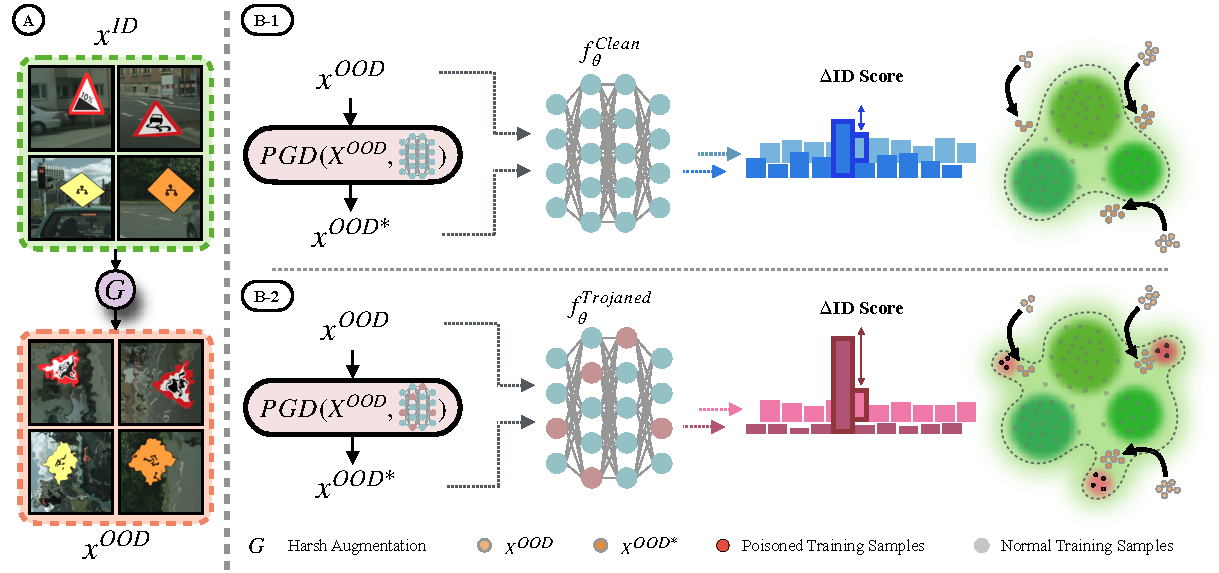
\includegraphics[width=1\linewidth]{Images/MainFigure.pdf}
    \caption{\textbf{An overview of TRODO} A) If a small portion of benign training samples was available, a module shown as \textbf{G} is used to obtain near-OOD samples. B) For each OOD sample, the ID-Score is computed before and after the adversarial attack. The difference between these scores is used as a signature to distinguish between a clean and a trojaned classifier. Performing the adversarial with not a large budget helps to discriminate between benign and trojaned classifiers 1) Lack of blind spots in the learned decision boundary of a clean model, makes it difficult to increase the ID-Score of OOD samples, resulting in small change in ID-Score. 2) For a trojaned model, $\Delta \text{\textbf{ID-Score}}$ is more discernible. This is due to the presence of blind spots, making it easier to shift OOD samples inside the decision boundary.}
\label{MainFigure}
    
    \vspace*{-6mm}

  \end{center}
\end{figure*}



% \begin{figure*}[t]
%   \begin{center}
%     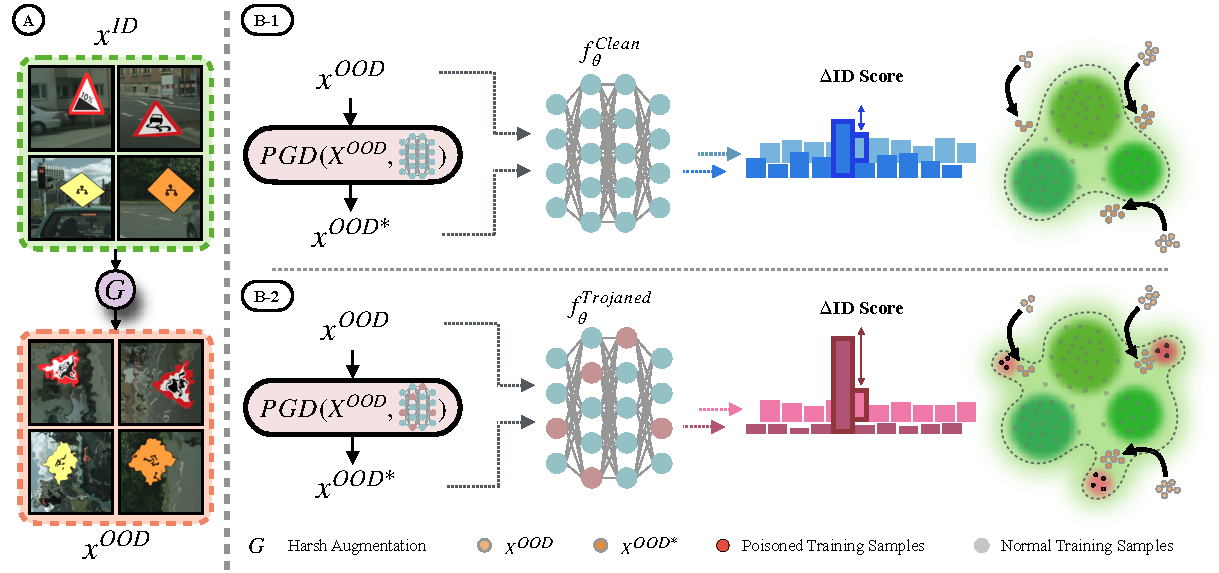
\includegraphics[width=1\linewidth, bb=0 0 600 280]{Images/MainFigure.pdf}
%     \caption{\textbf{An overview of TRODO} A) If a small portion of benign training samples was available, a module shown as \textbf{G} is used to obtain near-OOD samples. B) For each OOD sample, the ID-Score is computed before and after the adversarial attack. The difference between these scores is used as a signature to distinguish between a clean and a trojaned classifier. Performing the adversarial with not a large budget helps to discriminate between benign and trojaned classifiers 1) Lack of blind spots in the learned decision boundary of a clean model, makes it difficult to increase the ID-Score of OOD samples, resulting in small change in ID-Score. 2) For a trojaned model, $\Delta \text{\textbf{ID-Score}}$ is more discernible. This is due to the presence of blind spots, making it easier to shift OOD samples inside the decision boundary.}
%     \label{MainFigure}
%     \vspace*{-6mm}
%   \end{center}
% \end{figure*}

\section{Related Work}
% \textbf{Backdoor Attacks.}\ \ Injecting pre-defined triggers into the training data is the most common approach to implement backdoor attacks. BadNet \cite{badnets} is the first backdoor attack against DNN models, which involves modifying a clean image by inserting a small, predetermined pattern at a fixed location, thus replacing the original pixels. Blended \cite{blended} aimed to enhance the invisibility of the trigger pattern by seamlessly blending it into the clean image through alpha blending. SIG \cite{sig} utilized a sinusoidal waveform signal as the trigger pattern. To achieve better stealthiness, many attacks with invisible and dynamic triggers have been proposed. Input-aware \cite{inputaware} proposed a training-controllable attack method that simultaneously learned the model parameters and a trigger generator to produce a unique trigger pattern for each clean test sample. For more details regarding other attacks including BPP \cite{bpp}, SSBA \cite{ssba}, WaNet \cite{wanet}, and \cite{color} read Appendix Section \ref{app:backdoor-attacks}.


\textbf{Trojan Scanning.}\ \ Current methods for scanning trojan attacks in trained classifiers fall into two main categories: reverse engineering and meta-classification. Reverse engineering methods, such as NC \cite{NC}, ABS \cite{ABS}, TABOR \cite{TABOR}, PTRED \cite{PTRED}, and DeepInspect \cite{DeepInspect}, identify trojaned models by applying and optimizing a trigger pattern to inputs, causing them to predict the trojan label. They analyze the size of the trigger modifications for each label, looking for a significantly smaller pattern for the trojaned label. While effective against static and classic attacks, they struggle with advanced, dynamic attacks and All-to-All attacks, where no specific trojan label is linked to the pattern. UMD \cite{umd} attempts to detect X2X attacks but is limited to specific types and single trigger patterns. FreeEagle \cite{freeeagle} optimizes intermediate representations for each class and scan for a class with particularly high posteriors, if any. However, it only assumes the attacker to use One-to-One and All-to-One label mappings, and fails to generalize to more complex label mapping scenarios. Meta-classification detector methods like ULP\cite{ULP} and MNTD \cite{MNTD} train a binary meta-classifier on numerous clean and trojaned shadow classifiers to learn distinguishing features. These methods perform well on known attacks but fail to generalize to new backdoor attacks and require extensive computational resources to train shadow models \cite{xiang2024cbd}. Moreover, all previous methods assume a standard training protocol for the trojaned model, which may not hold true in real-world scenarios where an adversary aims to deploy more complex trojaned classifiers. By implementing adversarial training on poisoned training data, the effectiveness of previous methods, which rely on exploiting known signatures, may be compromised, as observed by \cite{odyssey,zhang2021cassandra}. 

% Maybe should be added later

% Many other recent methods have been proposed as well \cite{hou2024ibd, qu4821388input, zhu2024neuralsanitizer, guan2024ufid, cheng2024lotus, lyu2024task, zhu2024seer, murad2024advancing}.

\textbf{ID-Score and OOD Detection Task.}\ \  A classifier trained on a closed set, can be utilized as an OOD detector by leveraging its confidence scores assigned to input test samples, referred to as ID-Score in this study. Here, the closed set is the training set used for the classification task, and the samples within this set are called ID samples. Various strategies have been proposed to compute ID-Scores from a classifier, among which the MSP has proven to be an effective and general scoring strategy compared to others \cite{liang2017enhancing,kong2021opengan,fort2021exploring,hendrycks2016baseline,ruff2021unifying,salehi2021unified}. The classifier assigns higher ID-Scores to samples that belong to the ID set and lower scores to OOD samples. In this study, we have adopted MSP as our ID-Score based on its demonstrated efficacy in OOD detection literature \cite{msp} and its constrained range between $(0.0, 1.0)$, unlike other ID-Score methods such as KNN distance \cite{sun2022out}, which do not have defined upper and lower bounds. We consistently employ MSP in our methodology, hypothesizing that an MSP value of 0.5 (we call this value boundary confidence level and denote it as $\gamma$) signifies regions near the classifier's decision boundary. Notably, our study includes a comprehensive ablation study of this hyperparameter, detailed in Table \ref{tab:bcl}.






% Current techniques for determining if a trained classifier has been compromised by a backdoor attack are primarily divided into two main groups. Detectors based on reverse engineering and detectors based on Meta-classification. Reverse engineering approaches \cite{NC, ABS, TABOR, PTRED, DeepInspect} specifically identify trojaned models by applying a short-cut modification (i.e. the trigger pattern) to inputs causing them to be predicted as the trojan label. subsequently, these methods calculates such modification through optimization for each label and analyzes if there is a short-cut which is much smaller in size than the modifications of other labels. These approaches while effective on static and classic attacks, fall short in detecting advanced and dynamic attacks. These methods are unable to detect All-to-All attacks where the pattern itself does not lead to a specific trojan label, as the shortcut no longer exists in such cases. However, while UMD \cite{umd} attempts to detect any X2X attack, it only considers limited types of attacks and those with only one trigger pattern.  
%  Meta-classification detectors \cite{ULP, MNTD}  train a binary meta classifier on a large number of clean and trojaned shadow classifiers for learning the distinguish features between two set. Although these methods are effective on the seen attacks during training, they can not generalize to unseen backdoor attack. Additionally, training the shadow networks is computationally intensive. Moreover, all these methods assume a standard training protocol for the trojaned model, which may not hold true in real-world scenarios where an adversary aims to deploy more complex trojaned classifiers. By implementing adversarial training on poisoned training data, the effectiveness of previous methods, which rely on exploiting known signatures, may be compromised, as observed by \cite{odyssey,zhang2021cassandra}. For more details on baselines, refer to Appendix Section\ref{app:baselines}.
 
%  Additionally, these approaches presume standard training of the trojaned model and may not perform well under adversarial training conditions. As adversarial training alters the decision boundaries, makes distribution shifting difficult due to increased robustness.

 
%  Odyssey \cite{odyssey,zhang2021cassandra} also acknowledges this limitation, failing to handle adversarially robust training effectively due to the changed decision boundaries. For more details on baselines, refer to Appendix Section\ref{app:baselines}.
  
 % most scanning methods struggle to modify source class samples to be predicted as another class. 

% The OOD detection task refers to identifying samples that diverge from ID. practically previous works formulate the OOD detection task by considering two datasets $D$ and $D'$ respectively as the source of ID and OOD data samples (e.g. CIfar10 vs. Cifar100 task). During training,  dataset $D$, with labels are available, is used. In most previous works \cite{kong2021opengan,fort2021exploring,hendrycks2016baseline}, the detector $f$ is trained on the task of classifying ID classes. An OOD detector operates by assigning an OOD score to an input sample, where a higher score corresponds to OOD samples. The main challenge in OOD detection is finding an ideal score function that can assign scores to separate ID and OOD samples effectively. Existing score functions for an input test sample $x$ operate on the logits of $f(x)$, hypothesizing that OOD sample logits differ from ID ones. Typically, OOD samples' logits are more uniform because they are unseen by $f$ \cite{ruff2021unifying,salehi2021unified}.


\textbf{Adversarial Risk.}\ \ Adversarial risk refers to the vulnerability of machine learning models to adversarial examples \cite{pmlr-v80-uesato18a, pmlr-v89-suggala19a}. Previous work has established bounds on this metric via function transformation \cite{khim2019adversarial}, PAC-Bayesian \cite{pmlr-v238-mustafa24a}, sparsity-based compression \cite{balda2019adversarial}, optimal transport and couplings \cite{pmlr-v119-pydi20a}, or in terms of input dimension \cite{simon2019first}. This metric has been studied in the context of OOD generalization as well \cite{zou2024adversarial, fort2022adversarial, augustin2020adversarial}. High lower bounds of the metric have also been proved under some conditions such as benign overfitting for linear and two-layered networks \cite{hao2024surprising}.

For an extended related work, see Appendix Section \ref{ext_rel}.

 
% WaNet is  sample-specific
% backdoor attack that  uese the image warping technique as triggers



% BppAttack crafted poisoned images by exploiting color quantization, leveraging imperceptible image distortions as triggers.



% Generally, backdoor attacks are based on the assumption that an adversary can only modify a small fraction of the training data, and the model is then trained  poisoned training dataset by a regular training methods 




%     Gu et al. \cite{gu2017badnets} were the first to demonstrate a backdoor attack on deep neural network (DNN) models, using pixel modifications as a trigger that, while noticeable to humans, initiated a new era in stealthier attack methodologies. Advances in this area have led to two main strategies for hiding these triggers. Invisible triggers, which are subtle changes hard to detect by eye by minimizing the differences in pixels between altered and original images\cite{li2020invisible, chen2017targeted, zhong2020backdoor}, including techniques that maintain similarity in the model's internal representations of both\cite{doan2021backdoor, zhao2022defeat}; and natural triggers, which subtly alter the image's style to appear normal, employing methods like mimicking natural reflections \cite{liu2020reflection}, using social media-style filters\cite{liu2019abs}, applying generative adversarial networks\cite{cheng2021deep}, or performing image transformations\cite{nguyen2021wanet}. A common factor between all of these attacks is focusing on saving clean classification accuracy while achieving a high attack success rate (ASR), which measures the percentage of predicting attack target labels when adding a trigger to an image from another class, but in this work, we focus on out-of-distribution detection of backdoor attacks, and therefore we use other metrics explained in  

\begin{figure*}[t]
  \begin{center}
    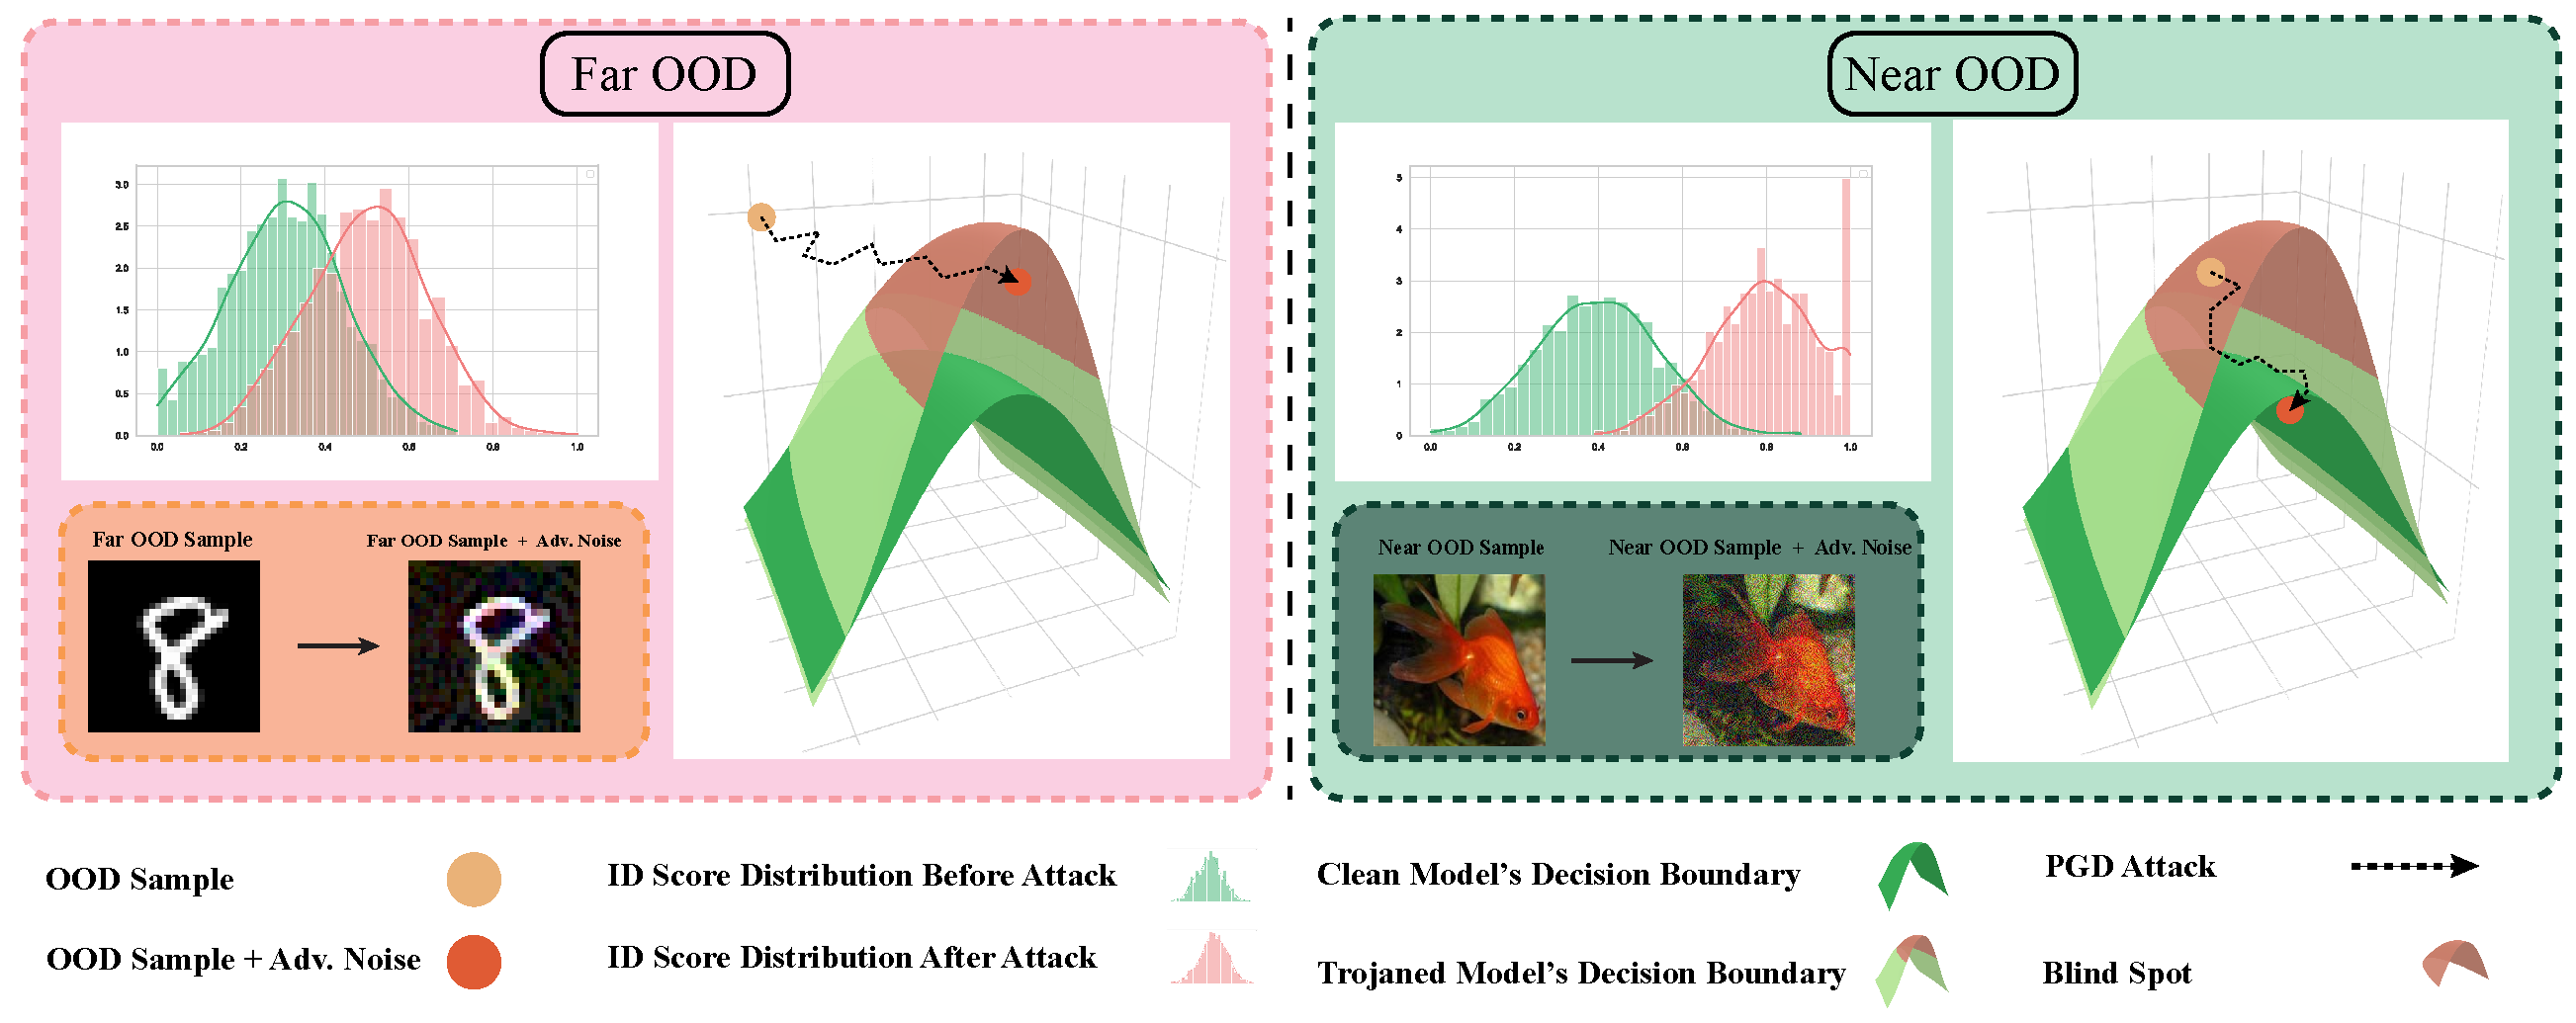
\includegraphics[width=1\linewidth]{Images/3dplot.pdf}
    \caption{\textbf{The effect of using near-OOD samples} Given a trojaned classifier trained on CIFAR10, due to the presence of blind spots in the learned decision boundary, it is easier to increase the ID-Score of near-OOD samples (a fish is considered as near-OOD for CIFAR10) than that of far-OOD samples (samples from MNIST are far-OOD for CIFAR10). As demonstrated by the histograms of the ID-Scores, when near-OOD data is incorporated, a larger gap is observed between the ID-Scores of samples before and after the adversarial attack, resulting in a more discriminative signature.}
\label{blindspot}

    \vspace*{-4mm}
    \label{fig:accs}

  \end{center}
\end{figure*}
\section{Threat Model}
\label{threat}

\subsection{Attacker Capabilities and Goals}
In the context of attacker capabilities, adversaries can poison training data \cite{badnets, blended} or manipulate the training process \cite{wanet, inputaware} to embed backdoors within models. They deploy triggers that vary from stealthy, undetectable modifications to overt ones, with triggers influencing either specific parts of a sample \cite{badnets, inputaware} or the entire sample \cite{sig, bpp}. Additionally, attackers can target individual samples \cite{ssba} to evade detection or use label-consistent mechanisms, where poisoned inputs align with their visible content, leading to inference misclassification \cite{turner2019label, sig}. Attacks typically follow either an All-to-One pattern, where any input with a trigger is classified into a single target class, or an All-to-All pattern, where a target class is chosen for each source class to ensure any input with a trigger is misclassified accordingly. These models may be trained either adversarially or non-adversarially, with attackers aiming to embed undetectable backdoors that evade detection efforts. 

\subsection{Defender Capabilities and Goals}
In contrast, defenders operate under varying capabilities: The defender receives the model with white-box access to it and may (TRODO) or may not (TRODO-Zero) have access to a small set of clean samples from the same distribution as the training data, and they require no prior knowledge of the specific attack type or trigger involved. Defender goals are to identify any embedded backdoors, and adapt effectively to scenarios with or without clean training samples.



\section{Method}


\textbf{Overview.}\ \ In this section, we describe the components of TRODO, which employs an adversarial attack (here we use PGD \cite{pgd}) to increase the ID-Score of OOD samples to shift them towards the training data distribution. We then measure the magnitude of the difference in ID-Scores between OOD samples and their perturbed counterparts. We denote this as the ID-Score difference ($\Delta \text{ID-Score}$) and use it as a signature to scan for trojans. This signature is more discriminative between clean and trojaned classifiers when near-OOD samples are used (See Figure \ref{fig:nearood} for some samples). Unlike many existing trojan scanners, which fail in setups lacking training data, TRODO can successfully conduct scans owing to its robust and universal signature. Further details are provided in subsequent sections. The pseudocode of our scanning algorithm is provided in \ref{app:alg}. 

\subsection{Design and Definition of TRODO's Signature}
 \textbf{OOD Set Crafting.} 
To obtain a set of OOD samples, we propose two scenarios. In the first scenario, a portion of the clean training data is available for the given classifier. Here, the OOD set is obtained by applying transformations known to compromise the semantic integrity of an image. Although the results of these transformations deviate from the ID characteristics, these transformed samples visually resemble ID ones. We utilize these as proxies for near-OOD samples. To ensure that the transformations significantly alter the sample characteristics and shift them far enough from the training data distribution, we define a set of hard transformations \(\mathcal{T} = \{T_i\}_{i=1}^{k}\), with each \(T_i\) representing a specific type of hard augmentation. For each ID sample \(x\), a random permutation of \(\mathcal{T}\) is selected \(\{T_{j_1},T_{j_2},\ldots,T_{j_k}\}\), and the transformations are sequentially applied, resulting in \(T_{j_k}(\ldots T_{j_1}(x))\). This method generates a diverse set of OOD samples, particularly valuable in environments with limited access to training data. Each transformed training sample \(x\) becomes a crafted OOD sample \(x'\), with the transformation process denoted by \(G(\cdot)\), i.e., \(x' = G(x)\). We set $k=3$ as a rule of thumb. For more details on these hard transformations, refer to Appendix Section \ref{sec:nearood}.
In the second scenario, where no training data is available, we employ a smaller dataset as the OOD set. Specifically, we utilize Tiny ImageNet \cite{imagenet} for this purpose. Considering that many training datasets (e.g., CIFAR-10 \cite{cifar}) share concepts with our OOD set, we apply \(G(\cdot)\) on Tiny ImageNet samples before using them as the OOD set, ensuring that they do not reflect the training distribution characteristics. In scenarios where a small portion of clean training data is available, we call our method \textbf{TRODO}, and when there is no access to training data, it is referred to as \textbf{TRODO-Zero}.


\textbf{Adversarial Attack on ID-Score.}\ \ In this section, we formulate an adversarial attack on OOD samples to shift them toward the ID region. First, we define the maximum softmax probability (MSP) as the ID-Score, which is an indicator of the classifier's confidence in recognizing an input sample belonging to the ID. Noteworthy that it has been shown that MSP is a simple yet effective metric to be used as ID-Score \cite{msp}. The adversarial perturbation aims to find a shortcut path to increase the ID-Score, effectively shifting the OOD sample toward the blind spots of the trojaned classifier. This process results in a significant increase in the ID-Score, highlighting the introduced signature. Formally, the PGD attack to the ID-Score for a sample $x$ corresponding to a classifier $f$ can be formulated as:
{\small
\begin{equation}
J(f(x)) = \text{ID-Score}_{f}(x), \quad
    x^{0*} = x, \quad 
    x^{t+1*} = \Pi_{x+\mathcal{S}} (x^{t*} + \alpha \cdot \text{sign}\left(\nabla_x J(f(x^{t*}))) \right), \quad
    x^{*} = x^{N*}
    \label{eq:pgd_attack}
\end{equation}}


where the noise is projected on the $\ell_{2}$ norm ball $\mathcal{S}$ with radius $\epsilon$ around $x$ in each step: $ \|x^{t*} - x\|_2 \leq \epsilon$.

To define our signature, we assume a set of OOD samples denoted as $D_{\text{OOD}} = \{ x_i^{\text{OOD}} \}$ is available. For a given classifier $f$, we define our signature $S(f, D_{\text{OOD}})$ as:

{\small
\begin{equation}
    S_i(f, D_{\text{OOD}}) = 
    \text{ID-Score}_{f}(x_i^{\text{OOD*}}) - \text{ID-Score}_{f}(x_i^{\text{OOD}}), \ \ \ 
    S(f, D_{\text{OOD}})=\frac{\sum_{i=1}^{|D_{\text{OOD}}|} S_i(f, D_{\text{OOD}})}{|D_{\text{OOD}}|}
    \label{eq:signal}
\end{equation}}

where $x_i^{\text{OOD*}}$ is obtained by adding adversarial perturbation to $x_i^{\text{OOD}}$ via a PGD attack mentioned in above equation \ref{eq:pgd_attack}.

A higher value of $S(f, D_{\text{OOD}})$ indicates that $f$ is trojaned with higher probability. To detect whether a classifier $f$ is trojaned, we utilize a validation set and a thresholding mechanism, which is well described in the next part. 

\subsection{Validation Data Utilization in TRODO}

\textbf{Leveraging Validation Set for Trojan Scanning.} \ \
In this study, we assume access to a benign validation set denoted as $D_v$ (e.g., Tiny ImageNet), which is realistic given the abundance of available datasets in real-world scenarios. We craft an OOD set $D_{\text{OOD}}$ by applying the mentioned strategy, i.e., $D_{\text{OOD}} = G(D_v)$. Note that we apply harsh augmentations to ensure that the OOD dataset does not belong to ID (in case the validation dataset's distribution resembles training data distribution). These datasets are used for computing $\epsilon$ for our Projected Gradient Descent (PGD) attack as mentioned in the above equations. Moreover, leveraging them, we propose a threshold mechanism to determine whether an input classifier is trojaned, using the signature $S(f, D_{\text{OOD}})$.


Initially, we note that the ID-Score of an OOD sample \(x\) resembles a uniform distribution \(\mathcal{U}(K)\), and the \(\text{ID-Score}_f(x_{\text{OOD}})\) is approximately equal to \(\frac{1}{k}\), where \(k\) denotes the number of classes in the training data. We propose that an effective \(\epsilon\) should shift OOD samples toward ID regions. We consider 0.5 as a hyperparameter, denoted by \(\gamma\), which we refer to as the boundary confidence level. As a result, we propose computing \(\epsilon\) by finding the minimum perturbation that can increase the ID-Score (i.e., MSP) from \(\frac{1}{k}\) to 0.5 for the crafted OOD set \(D_{\text{OOD}}\), corresponding to a surrogate classifier \(g\) as a clean trained model. Specifically, we use the method proposed in DeepFool \cite{deepfool} to find the minimum perturbation that can satisfy the mentioned constraint:
{\small
\begin{equation}
 \quad \epsilon = \arg \min_{\delta} \|\delta\|_{2} \quad \text{subject to } \quad \frac{ \sum_{x\in D_{\text{OOD}}}{\text{ID-Score}_{g}(x + \delta)}}{|D_{\text{OOD}}|} \ge \gamma.
\end{equation}
}
\textbf{Threshold Computing.} \ \
Once the signature value \( S(f, D_{\text{OOD}}) \) has been computed for the given classifier \( f \), it is critical to determine whether \( f \) has been compromised by a trojan, using a threshold-based strategy. This process is achieved by employing a statistical test on a set of scores computed for a surrogate classifier \( g \). Specifically, given the surrogate classifier \( g \) and the OOD set \( D_{\text{OOD}} \), we generate a set of baseline scores denoted as \(\{ S_i(g, D_{\text{OOD}})\}_{i=1}^{N} \). These scores represent the signature values assigned by a clean classifier \( g \). For the input classifier \( f \), we calculate its signature using the formula described in Equation \ref{eq:signal}. When the model is trojaned, its corresponding signature will be an outlier to the distribution of \( S_i(g, D_{\text{OOD}}) \).
We estimate this null distribution with a Normal distribution to find a threshold $\tau$ satisfying \(Prob(\underset{i=1,\ldots,N}{max} -log(1 - S_i(g, D_{\text{OOD}})) \leq \tau) > 0.95 \). Solving for $\tau$, gives the following threshold: $\tau = \Phi^{-1}_{\text{}}(\sqrt[N]{0.95})$, where $\Phi$ is the CDF of our estimated truncated normal distribution and we set $N=50$. We refer to $\tau$ as 
\textbf{scanning threshold}.

% {\small
% \begin{equation*}
%  \tau = \Phi^{-1}_{\text{}}(\sqrt[N]{0.95}),
% \end{equation*}
% }
% \kian{I suggest putting a pseudocode (1 or 2 algorithm boxes) to explain the method. right now the reviewer needs to read two pages to understand the trojan detection algorithm and it is confusing.} 
% \ali{We are going to do this, but it won't fit in main pages. We will provide it in Appendix.}
% \textbf{Shifting OOD Samples as a Signature}



% By applying a common attack such as PGD on OOD samples to adversarially increase their ID-Scores, we shift these samples toward the training data distribution. 




% \textbf{Threshold} \ \ % Definition of the threshold for detecting backdoored models
% \bd{
% In this study, we define the detection threshold \(\theta\) as \(\theta = \mu - z_{0.95} \times \sigma\), where \(\mu\) and \(\sigma\) represent the mean and standard deviation of the scores \(S\) from models trained under standard conditions. The value \(z_{0.95}\) corresponds to the critical z-value for a significance level of \(\alpha = 0.05\), typically associated with the 95\% confidence interval under the null hypothesis ($H_0$) that the model is not backdoored. A score \(S\) that results in a p-value less than \(\alpha\) suggests rejection of $H_0$, indicating anomalous behavior consistent with a backdoor.
% }




% In this section, we describe the use of the DeepFool attack to find an effective perturbation that leads to an error for a specific objective function. DeepFool is an iterative attack designed to find the minimal perturbation required to change the classification of a given sample.

% Let $f: \mathbb{R}^n \rightarrow \mathbb{R}^m$ be a classifier, where $f(x)$ denotes the output of the classifier for input $x$, and let $L$ be the objective function. The goal of DeepFool is to find the smallest perturbation $\delta$ such that the perturbed input $x + \delta$ is misclassified.

% The DeepFool algorithm proceeds as follows:

% 1. Initialize the perturbed sample as $x_0 = x$.
% 2. For $t = 0, 1, 2, \ldots$ until convergence, compute the perturbation $\delta_t$:
%     \begin{equation}
%     \delta_t = - \frac{f(x_t)}{\|\nabla f(x_t)\|_2^2} \nabla f(x_t),
%     \end{equation}
%     where $\nabla f(x_t)$ is the gradient of the classifier at $x_t$.
% 3. Update the perturbed sample:
%     \begin{equation}
%     x_{t+1} = x_t + \delta_t.
%     \end{equation}
% 4. Check if $f(x_{t+1}) \neq f(x)$. If so, stop the iteration and set $\delta = \sum_{i=0}^{t} \delta_i$.

% The resulting perturbation $\delta$ is the minimal perturbation required to change the classification of $x$ under the objective function $L$. This can be formally expressed as:
% \begin{equation}
% \delta = \arg \min_{\delta'} \|\delta'\|_2 \quad \text{subject to} \quad f(x + \delta') \neq f(x).
% \end{equation}

% Using the DeepFool attack, we effectively identify perturbations that exploit the vulnerabilities of the classifier with respect to the objective function $L$, leading to a misclassification.














% ****
% for computing $\epsilon$ for adverserial attack on OOD samples, we first train a surrgate classifier $g$ on   $D_{v}$ to obtain a  clean well-trained classifer. 


% specificly for computing $\epsilon$ we train a surrgate classifier $g$ on   $D_{v}$ to obtain a  clean well-trained classifer. 

% \begin{equation}
% \delta = \arg \min_{\delta'} \|\delta'\|_{2} \quad \text{subject to} \quad f(x + \delta') \neq f(x).
% \end{equation}



% it worth noting the logits of an OOD sample \(x\) resemble a uniform distribution \(\mathcal{U}_K\) and \({\text{ID-Score}}_{f}(x_{\text{OOD}}) \approx \frac{1}{k}\). To formulate attack on OOD sample   \(x_{\text{OOD}}\) to shifted to in-distribution, we aim to increase \({\text{ID-Score}}_{f}(x_{\text{OOD}})\) up to \(\frac{1}{2}\). 


% This corresponds to the classifier model \(f\)  recognize \(x_{\text{OOD}}\) with significant confidence as ID.   


% noteworthy there have many other metric as OOD score which are mostly based on last layers features and logits including KNN distance, mahalanobis distance, ODIN. in this study we considered ${\text{MSP}}_{f}(x)$ as our default posthoc method for detecting OOD data ability of classifier, however other scoring strategy have been explored.  \ali{nigga what? ablation miarim?}(see section X).




% This shortcut path is created by directing the optimizer to craft a perturbation that acts as a proxy for triggers, even when they are not explicitly available. As a result, a PGD attack with the same budget leads to a significant increase in the ID-Score for perturbed OOD samples in a trojan classifier compared to clean ones. 


% We denote a perturbed version of the OOD sample \(x^{\text{OOD}}\) as \(x^{\text{OOD*}}_f\). Then we define our signature for a classifier \(f\) as: 

% $\quad \quad \quad \quad \quad \quad  \quad \quad S(f,x^{\text{OOD}}) = \text{ID-Score}_{f}(x^{\text{OOD*}}) - \text{ID-Score}_{f}(x^{\text{OOD}})$  

% \frac{\sum_{i=1}^{|D_{\text{OOD}}|} (\text{ID-Score}_{f}(x_i^{\text{OOD*}}) - \text{ID-Score}_{f}(x_i^{\text{OOD}}))}{|D_{\text{OOD}}|}

% in this study we assume that there is an access to a benign validation set denoted as $D_{v}$ (i.e. tiny Imagenet), which holds in real world scenario where there are tons of availble datasets. we craft a OOD set $D_{\text{OOD}}$  by applying mentioned strategy  i.e. $D_{\text{OOD}}=G(D_{\text{v}})$ 
% we use theses dataset for computing $\epsilon$ of our PGD attack mentioned in above equtions. morever leveraging them we propse a threshold mechanism to determine wether an input classfier is trojaned, using its signiture $S(f, D_{\text{OOD}}) $. 


% at first we note that the logits of an OOD sample \(x\) resemble a uniform distribution \(\mathcal{U}_K\) and \({\text{ID-Score}}_{f}(x_{\text{OOD}}) \approx \frac{1}{k}\) where $k$ denotes the number of classes of training data. we propose an effective $\epsilon$ should shift OOD samples toward ID regions significantly. as a result we propose computing $\epsilon$ by founding which value of that could increase ID-Score  from $\frac{1}{2}$ to $0.5$  for OOD set  $D_{\text{OOD}}$ corresponding to surrogate classifier $g$. specificly we use Deepfool attack to find the minimum purtubation that can satisfy the mentioned constraint:
% \begin{equation}
% \text{For} \ x \ in \ D_{\text{OOD}}:  \ \delta = \arg \min_{\delta'} \|\delta'\|_{2} \quad \text{subject to  } \quad \text{ID-Score}_{g}(x) \approx 0.5. 
% \end{equation}

% after computing those purtubation for each OOD sample we use 


% To formulate attack on OOD sample   \(x_{\text{OOD}}\) to shifted to in-distribution, we aim to increase \({\text{ID-Score}}_{f}(x_{\text{OOD}})\) up to \(\frac{1}{2}\). 
% give a signiture value has been achived for input classifier $f$ , we need to determine wether it has been trojaned base  threshold strategy.  we over come this by using statistical test on set of computed scores for $g$. specificly given surrogate classifier $g$ and OOD set $D_{\text{OOD}} $ we creat a set of scores denoted as $S(g, D_{\text{OOD}})$ corresponding to signitures value assigned by a clean classiferi $g$. for an input classifier $f$ we compute its signture using \ref{eq:signal} then given $S(g, D_{\text{OOD}})$ we determined if the $f$ is trojaned by applying statstical test between them.

% In this section, we formulate an adversarial attack on OOD samples to shift them towards the ID region. First, we define the maximum softmax probability (MSP) as the ID-Score, which is an indicator of the classifier's confidence in recognizing an input sample as belonging to the ID. The crafted perturbation aims to find a shortcut path to increase the ID-Score, effectively shifting the OOD sample towards the blind spots of the trojaned classifier. This process results in a significant increase in the ID-Score, highlighting the introduced signature.   Formally PGD attack to ID-Score for a  sample $x$ corresponsinf to a classifier $f$ could be formaluated as:

% $  x_{0}^{*} = x, \quad \quad x_{t+1}^{*} = x_{t}^{*} + \alpha \cdot \text{sign}\left(\nabla_x  J(f(x_{t}^{*})) \right),  \quad \quad  x^{*}=x_{N}^{*},  \quad \quad J(f(x)) = -\text{ID-Score}_{f}(x)$.
% where  the noise is projected within the \(\ell_{2}\) norm in each step: $\|x - x_0\|_2 \leq \epsilon$. 

% to define our signiture we assume a set as source of OOD sample denoted as $D_{\text{OOD}}=\{ x_i^{\text{OOD}} \}$ is availble, where for   considering $f$ 

% we will define our signiture   $S(f,x^{\text{OOD}})$ as:

% $\quad \quad \quad \quad  \quad \quad S(f,D_{\text{OOD}}) = \frac{\sum_{i=1}^{|D_{\text{OOD}}|}  ( \text{ID-Score}_{f}(x_i^{\text{OOD*}}) - \text{ID-Score}_{f}(x_i^{\text{OOD}}))}{|D_{\text{OOD}}|}$  where $x_i^{\text{OOD*}}$ have obtained by adding purtutabtion to $x_i^{\text{OOD}}$ by a  PGD attack.


%  which higher value for that indicate that $f$ is backdoored with higher probability. as we need a thresholding mechanism for detecting whether an input classifier $f$ is backdoored or not we utilize a validation set and a classifier as 

% . 

% $  x_{0}^{*} = x, \quad \quad x_{t+1}^{*} = x_{t}^{*} + \alpha \cdot \text{sign}\left(\nabla_x  J(f(x_{t}^{*})) \right),  \quad \quad  x^{*}=x_{N}^{*},  \quad \quad J(f(x)) = -\text{ID-Score}_{f}(x)$


  
% we use a valition set as source of OOD data and if training samples are areplace them with near OOD data


% to create OOD set, In scenarios where  a limited number of trained samples are available, we transform them with hard augmentation to generate related OOD samples. otherwise we use which leads to a more discriminative signature. Otherwise, we use a validation set as the OOD set. 


% 


% scanning for \textbf{\textit{TRO}}janed Models via \textbf{\textit{D}}etection of Adversarial Shifts in Near \textbf{\textit{O}}OD Samples (TRODO) where in

 % $ x^*_{\text{OOD},0} = x_{\text{OOD}},  \quad \quad  \quad  x^*_{\text{OOD}, t+1} = x^*_{\text{OOD}, t} + \alpha \cdot \text{sign}(\nabla_{x} J(f(x^*_{\text{OOD}, t}))), \quad \quad  x^*_{\text{OOD}} = x^*_{\text{OOD}, N}$

% denoted as ${D^{OOD^*}_{f}}$ in this study. using a validation set for creating a pool of $\{D^{OOD_i^*}_{f}\}$ corresponding to a  clean classifier f and set of OOD samples $\{OOD_i\}$, we compute  ${D^{OOD^*}_{g}}$ for a input classifier $g$ and with comparing $\{D^{OOD_i^*}_{f}\}$ determine wether $g$ is scanned.


% , we utilize the distance of shifted perturbed OOD samples as a signature to indicate whether a classifier has been Trojaned. Specifically, this signature is more pronounced when OOD samples are near the in-distribution boundary. We utilize this signature to scan an input model to determine whether it is backdoored, specifically for a given classifier \( f \) and samples \( \{x^i_{\text{ID}}\} \) that belong to the training set \( D \). We craft near OOD samples by applying \( G(.) \), reaching \( \{x^i_{\text{OOD}}\} = G(\{x^i_{\text{ID}}\}) \). Due to the strategy mentioned in Section X, by adding perturbation to OOD samples \( \{{x^{i*}}_{\text{OOD}}\} \), we create adversarial OOD samples. The feature space distance between them, i.e., \( J(f(x^*_{\text{OOD}}) \| f(x_{\text{OOD}})) \), is used as a signature. Here, \( J(\cdot \| \cdot) \) is the Jensen-Shannon divergence, a symmetric version of the Kullback-Leibler divergence, commonly used to compute the distance between two distributions.  
% $$\text{KL}(P \parallel Q) = \sum_{i} P(i) \log\left(\frac{P(i)}{Q(i)}\right), J(P \| Q) = \text{KL}(P \parallel Q) + \text{KL}(Q \parallel P) $$

% Formally we consider the $J(f(x^*_{\text{OOD}}) \| f(x_{\text{OOD}})$  as an indicator which higher value for that indicate that $f$ is backdoored with higher probability. as we need a thresholding mechanism for detecting whether an input classifier $f$ is backdoored or not we utilize a validation set and a classifier as 



%  \textbf{validation set as OOD source}

% \textbf{validation set for backdoor model scanning}
% we consider a dataset as validation set were we train a clean classifier on that then utilize our proposed signature on that to exploit scanning score for a clean model. specifically we use tinyimagenet and train a classifier $f$  on that then by proposed strategy in section X we find scores correspond to a clean model.

% To obtain a set of OOD samples, we propose two scenarios. In the first scenario, there is access to a portion of the training data for the input test classifier. In this scenario, the OOD set can be generated by applying transformations known to be harmful for preserving the semantic integrity of an image, such as cutout. These transformations produce samples which, while not part of the ID, retain a degree of visual similarity to ID samples. In this study, we utilize such samples as a proxy for Near OOD samples. To ensure that these transformations meaningfully alter the characteristics of the samples, distancing them from the training data distribution, we define a set of hard transformations \(\mathcal{T} = \{T_i\}_{i=1}^{k}\), where each \(T_i\) represents a specific hard augmentation. For each ID sample \(x\), a random permutation of \(\mathcal{T}\) is selected, and the transformations are applied in a randomized sequence to the sample, producing \(T_{i_k}(\ldots T_{i_1}(x))\). This process is designed to craft a diverse set of OOD samples, especially useful in settings where access to the training set is limited. Each transformed training sample \(x\) results in a crafted OOD sample \(x'\), where the transformation process is denoted as \(G(\cdot)\), i.e., \(x' = G(x)\). regarding which hard transformation seleted please see appendix X. in other scanrio that there is no access to a training data we utilze a small dataset as OOD set. specificly we utilze tiny imagenet as OOD set for this setup. as may training data (e.g. CIFAR10) share some concept with our OOD set in secanrio we apply $G(.)$ on TinyImagnet before utilizing as OOD set, to ensure that they do not blong to training distribution.) we coin our method in supervised scenorio ad TRODO and unsupervised scenario as UNTRODO.




% This method systematically ensures that \(X'\) significantly diverges from the ID, validating their use as effective OOD samples. 


 


% In this section we explain compononets of TRODO. which using an algorithm attack such as PGD aims  increasing MSP score of OOD samples to shift toward training data distribution. in next step we measure magnituted of shifting distnace of purturbed OOD samples  compare to it clean counterpart denoted as in feature distance as a signiture. in scenario that evenv a limited of trained samples are availble we transform them with hard augmention as related OOD samples leads to more discriminative signutre. other wise we utilize a validation set as OOD set. more details have been provided in following.


% For an in-distribution sample \(x_{\text{ID}}\) and its adversarially shifted version toward in-distribution, denoted as \(x^*_{\text{OOD}}\), the feature space distance between them, i.e.,  \(J (x^*_{\text{OOD}}\| x_{\text{OOD}})\), could be used as a signature. Here, \(J (. \| .)\) is the Jensen-Shannon divergence, a symmetric version of the Kullback–Leibler divergence, commonly used to compute the distance between two distributions.

% We aim to adversarially move crafted near-OOD samples toward the in-distribution while shifting ID samples toward out-of-distribution using the PGD algorithm, by adding small perturbations at each step. Specifically, we target the MSP values of ID and OOD samples, aiming to decrease the MSP value for ID samples and increase it for OOD samples.

% Given an ID sample \(x\), we craft its OOD counterpart \(G(x)\) by applying the specified augmentations. We hypothesize that the vector between \(x\) and \(G(x)\) represents a transition from out-of-distribution to in-distribution. We further hypothesize that this vector in backdoored classifiers is more susceptible to change compared to clean models. This is primarily based on the intuition that backdoored models, through overfitting to triggered samples during training, show different generalization behavior. 

% By targeting MSP values, we aim to use adversarial strategies to manipulate the perceived distribution of samples, thereby testing the resilience of classifiers against such model manipulations.



% \textbf{shifting OOD samples as a signiture} \ \ motivated by mentioned insights in theoritical section we utilize shifted OOD samples distance as a signature of classifier is tronjaned. specificly this signiture is more highlighted  when OOD samples are near to in-distribution boundry. conditioning 
  
  
%   specificly for a $x_{\text{ID}}$ and its shifted version to in-distribution denoted as   $x^*_{\text{OOD}}$ the distance between them in feature space i.e. $J (x^*_{\text{OOD}} \| x_{\text{OOD}}) $ could be use as a signiture where $J (. \|.) $ is Jensen-Shannon divergence, which is a symmetric version of Kullback–Leibler divergence a common metric for computing distance between two distribution. 

  
% we aim to adverserially move crafted near OOD samples toward in-distribution  meanwhile shift ID samples twoard out-of-distribtion by PGD by  adding small purtubation with PGD algorithm in each step.  to do this we consider MSP of ID and OOD samples as target for shifting data, specficly we adverserially aim to decrease MSP value for ID samples and increase that for OOD samples:

 

 
% given an ID sample $x$, we craft its OOD-counter part $G(x)$  by applying mentioned augmentions. we hypothesize that the vector between $(x,G(x))$ represents a vector from out of the distribution to in-distribution. we hypothesis that this vector in backdoored classifiers are more vulnerable to change compare to clean models. this is mainly because based on the intuition that backdoored models generaliztion through overfitting to triggered samples during training cause. 
% we aim to adverserially move crafted near OOD samples toward in-distribution  meanwhile shift ID samples twoard out-of-distribtion by PGD by  adding small purtubation with PGD algorithm in each step.  to do this we consider MSP of ID and OOD samples as target for shifting data, specficly we adverserially aim to decrease MSP value for ID samples and increase that for OOD samples:

  

    



% ***********

%  $x$

%  $ \quad \quad  \quad \quad  \quad \quad x_{0}^{*} = x, \quad \quad x_{t+1}^{*} = x_{t}^{*} + \alpha \cdot \text{sign}\left(\nabla_x J\left( x_{t}^{*}, y\right)\right),  \quad \quad  x^{*}=x_{N}^{*}$







% Classifiers such as $f$ trained on a dataset like $D$ can be utilized as OOD detectors due to their learned features from $D$ samples. specificly another dataset with seperate semantics presented in $D$ denoted as $D'$ is assumed as source of OOD samples. for instance a classifer trained on $Cifar10$ is use to detect $Cifar100$ as OOD samples. the $D$ and $D'$ are refered as ID and OOD set as well. the instructions to practically do OOD detecin this is using the output distribution of a classifier over classes of $D$ for a given input, offering insights into the model's prediction confidence. specifily  It is observed that classifiers tend to be more confident about ID samples compared to OOD samples. The Maximum Softmax Probability (MSP) has been proposed as an indicator of this confidence.  


% Consider a well-trained classifier \(f_{\theta}\) on an ID set with \(k\) classes. The classifier's logits from its penultimate layer for a given input sample \(x\) are represented by \(z = f_{\theta}(x)\), where \(z\) is a vector of unnormalized prediction scores \([z_1, z_2, \dots, z_k]\) for each class. Applying the softmax function results in:
% \begin{equation}
% \text{softmax}(z_i) = \frac{e^{z_i}}{\sum_{j=1}^k e^{z_j}}, 
% \end{equation}
% for each class \(i\), where \(z_i\) is the logit corresponding to the \(i\)-th class. This function outputs a probability distribution \(p\) over the classes, where:
% $p_i = \text{softmax}(z_i) $. The ${\text{MSP}}_{f}(x)$ for the input sample \(x\) is determined by:
% \begin{equation}
% \text{MSP}(x) = \max(p) = \max_{i \in \{1, \dots, k\}} p_i
% \end{equation}












% The previous section provides an intuition about how classifiers can be fooled with an input sample \(x \in D\). Here, we aim to formulate adversarial attacks on OOD samples such as \(x \in D'\). Specifically, we target the MSP score for OOD samples, where an increase in \({\text{MSP}}_{f}(x)\) implies that the confidence of \(f\) regarding the classification of \(x\) as belonging to in-distribution increases. Intuitively, this type of attack shifts an OOD sample \(x\) into the in-distribution category by adding adversarial perturbations.

% Previous studies have shown that even classifiers adversarially trained on \(D\) (the in-distribution set) are vulnerable to adversarial perturbations on OOD samples, mistakenly classifying them as ID.


%  where previous section provides intution about how classfiers fool on input sample $x \in D$. here we aim to formulate adverserial attack on OOD samples such as $x \in D'$. to formulate this we target MSP score for OOD samples, where increasing ${\text{MSP}}_{f}(x)$  means that the  $f$ confidence regarding that $x$ belongs to in-distribution increases intutatively this kind of attack shift OOD sample $x$ in to in-distribution by adding adverserial purtubation.  previous studies have been show that even classfiers adversrially trained on $D$ (i.e. in-distribution set) are vulnerable to adverserial purtubation on OOD samples and consider them as ID. 



%  $$L(x,y,F)=:\mathds{1}[y=0].L_{\mathrm{CE}}\left(F\left(x\right), \mathcal{U}_K\right)-\mathds{1}[y=1].\sum_{i=1}^K F_i\left(x\right) \log F_i\left(x\right)$$ 

 

% we aim to adverserially move crafted near OOD samples toward in-distribution  meanwhile shift ID samples twoard out-of-distribtion by PGD by  adding small purtubation with PGD algorithm in each step.  to do this we consider MSP of ID and OOD samples as target for shifting data, specficly we adverserially aim to decrease MSP value for ID samples and increase that for OOD samples:

 

 
% given an ID sample $x$, we craft its OOD-counter part $G(x)$  by applying mentioned augmentions. we hypothesize that the vector between $(x,G(x))$ represents a vector from out of the distribution to in-distribution. we hypothesis that this vector in backdoored classifiers are more vulnerable to change compare to clean models. this is mainly because based on the intuition that backdoored models generaliztion through overfitting to triggered samples during training cause. 
% we aim to adverserially move crafted near OOD samples toward in-distribution  meanwhile shift ID samples twoard out-of-distribtion by PGD by  adding small purtubation with PGD algorithm in each step.  to do this we consider MSP of ID and OOD samples as target for shifting data, specficly we adverserially aim to decrease MSP value for ID samples and increase that for OOD samples:

% specificly for a ed

%  $$L(x,y,F)=:\mathds{1}[y=0].L_{\mathrm{CE}}\left(F\left(x\right), \mathcal{U}_K\right)-\mathds{1}[y=1].\sum_{i=1}^K F_i\left(x\right) \log F_i\left(x\right)$$ 


%  $$x_{0}^*=x, \quad \quad   x_{adv}^{(t+1)} = x_{adv}^{(t)} + \alpha \cdot \text{sign}\left(\nabla_x J\left(F\left(x_{adv}^{(t)}\right), y\right)\right)$$

%    $$x_{0}^*=x, \quad \quad   x_{adv}^{(t+1)} = x_{adv}^{(t)} + \alpha \cdot \text{sign}\left(\nabla_x J\left(F\left(x_{adv}^{(t)}\right), y\right)\right)$$
%  where  $\mathcal{U}_K$
%  is a uniform distribution.

 

 

% with crafting $X=X_{ID} \bigcup X_{OOD}, \quad  Y=(1\bigcup 0)$ and applying mentioned adverserial attack, targeting MSP for ID and OOD samples we reach purturbed version of them denoted as 

%  $X=X_{ID}^{adv} \bigcup X_{OOD}^{adv}$ 
%  we show observe that lack of robustness of backdoor model leads to its 



% $$v_1=X_{ID}^{adv}-X_{ID}  \quad v_2=X_{OOD}^{adv}-X_{OOD} $$




% $$v_1=X_{OOD} -X_{ID}  \quad v_2=X_{OOD}^{adv}-X_{ID}^{adv} $$

% \begin{equation}
%     J (v_1 \| v_2)=D_{\mathrm{KL}}(v_1 \| v_2)+D_{\mathrm{KL}}(v_2 \| v_1)
% \end{equation}



% we use  $J (v_1 \| v_2)$ as a measure of robustness of trageted classifier where larger value indicates the classifier is backdoored with higher probablity and lower valu indicates the classifier is clean and considered as a clean model  



% in many case there is no access to training samples  of a dataset in such cases as a result crafting OOD samples would be a challange. for those cases we propose utilizing a validation set as OOD and adapt metnioned eqution above for those secnario, to solely apply for OOD samples and consider change of distribution of OOD samples before and after adverserial attack as signiture.

% which means 

% $$v_1=X_{ID}^{adv}-X_{ID}  \quad v_2=X_{OOD}^{adv}-X_{OOD} $$

% \begin{equation}
%    D_{\mathrm{KL}}(v_2 \| v_1)
% \end{equation}



 
 
% post-hoc methods utilzes the logits or features extracted by  $f_{\theta}$ to distingushes OOD data from ID data. an   detector method by assigning OOD score to samples. ideally an OOD detectors assigned scores tottally distingushes two in- and out-of-distribution data.   


%  The 


% Considering ID samples include  we assume that 0.01 of trainig set samples 






 
% \textbf{Minimum Step to Shift ID samples.}
% It has been shown that DNNs are vulnerable to adverserial attacks.


%  \textbf{Adverserial Attack on  a classifiers }
%  It has been shown that DNNs are vulnerable to adverserial attack on various task, which mostly explored on classification task, where adverserial purtubation during inference added to input data to make classifier mispredict its label. in other word a purturbation such as $\delta$ is added to sample $x$ with label $y$ to fool model to output $\hat{y}$ for adverserial input sample $x^{*}$  where $x^{*}=x+\delta$. specificly PGD is a terative adverserial attack to craft adverserial attack where the noise should be projected in $\ell_{2}$:

%   $$x_{0}^*=x, \quad \quad   x_{t+1}^{*} = x_{t}^{*} + \alpha \cdot \text{sign}\left(\nabla_x J\left( x_{t}^{*}, y\right)\right)$$

% where   $ J\left( x_{t}^{*}, y\right) $  denotes the for targetting objective function where for classifyers is cross entropy.   

% previous studies has been shown that  standard trained classfiers  are vulnerable to   adverserial attack even waek attacks such as FGSM, and differnet kinds of defence mechanism have been proposed to tackle this, most effective adverserial training on $D$.


 
% =D_{\mathrm{KL}}(v_1 \| v_2)+D_{\mathrm{KL}}(v_2 \| v_1)

 

% The previous section provides an intuition on how a classifier could  misclassify a input sample x with adding adverserial purtutbation and targeting cross-entropy loss function. in this section we formulate adverserial attack to OOD samples to  move it toward the in-distribution. 
% Specifically, by targeting an increase in the MSP score for OOD samples,  the confidence of \(f\) in considering \(x\) as belonging to the in-distribution increases. at first step logits of an OOD sample $x$ is uniform like  $\mathcal{U}_K$ and \({\text{MSP}}_{f}(x_{\text{OOD}}) \approx \frac{1}{k}\). for ensuring  $x_{\text{OOD}}$ has been shifted to in-distribution we   increase \({\text{MSP}}_{f}(x_{\text{OOD}})\) up to $\frac{1}{2}$ which corresponds to that classifier model $f$ with significant confidence consider $x_{\text{OOD}})$ as in-distribution. in seek of 



% can be deceived by an input sample \(x \in D\)  .


% Specifically, by targeting an increase in the MSP score for OOD samples, these samples gradually move toward the in-distribution boundary.

% An increase in \({\text{MSP}}_{f}(x)\) suggests that the confidence of \(f\) in classifying \(x\) as belonging to the in-distribution increases.

% at first 


% We consider \({\text{MSP}}_{f}(x) = 0.5\) as a threshold for determining if a sample \(x\) is in-distribution.

% Intuitively, this type of attack shifts an OOD sample \(x\) into the in-distribution category by adding adversarial perturbations.

% Previous studies have demonstrated that even classifiers adversarially trained on \(D\) (the in-distribution set) are vulnerable to adversarial perturbations on OOD samples, mistakenly detecting them as ID.




% \textbf{ a Classifier as OOD data detector}

% it has been show that a classifier trained on training set (ID samples) could be utilize as a OOD sample detector owe to its learned features from ID samples. to identify data samples that deviate from the distribution the classifier was trained on it has proposed to utilize distribution provided by classifer in the final lyer  over classes for a given input. This distribution can give insights into how confident the model is about its predictions. it has been shown that a clissifier is more confident about ID samples compare to OOD samples, and one proposed maximum softmax probablity as an indicator of this confidnece.
% given that a classifier $f_{\theta}$ is well trained on a ID set with $k$-classes, post-hoc shows the classifeirs logits and it pneumlates layer would be a reprsentitve as a data belongs to ID data. specificly maximum soft max probablity value for a input sample $x$



%  specificly Maximum Softmax Probability (MSP) is used in the context of out-of-distribution (OOD) sample detection in  models, particularly classifiers. It leverages the softmax output probabilities to determine the confidence level of the predictions, aiding in distinguishing between in-distribution and out-of-distribution samples.

 
% consider   outputs logits \( z = f(x) \) for a given input sample \( x \). Here, \( z \) is a vector of unnormalized prediction scores \( z = [z_1, z_2, \dots, z_K] \) for each of the \( K \) classes.  by applying soft max function we will have:

%  \begin{equation}
% \text{softmax}(z_i) = \frac{e^{z_i}}{\sum_{j=1}^K e^{z_j}}
% \end{equation}
% for each class \( i \), where \( z_i \) is the logit corresponding to the \( i \)-th class. This function outputs a probability distribution \( p \) over the classes, where:
% \begin{equation}
% p_i = \text{softmax}(z_i)
% \end{equation}

%  The MSP for the input sample \( x \) is determined by:\begin{equation}
% \text{MSP}(x) = \max(p) = \max_{i \in \{1, \dots, K\}} p_i
% \end{equation}
% This represents the highest probability assigned to any class by the model, reflecting the confidence level of the model's prediction. 


% \textbf{Near OOD sample Generation.} In the field of Out-Of-Distribution (OOD) detection, it is generally presumed that the training dataset \(\mathcal{D}_{\text{train}}\) solely comprises In-Distribution (ID) samples. If we have access to a subset of this dataset, denoted as \(X\), we can generate pseudo-OOD samples, \(X'\), by applying hard transformations that are known to be harmful to semantic preserving, such as cutout. These transformations craft samples that, although not belonging to the ID, retain a degree of visual similarity to ID samples, considering them as Near OOD samples, which means play as place holder for boundry of distribution of training set.






% To ensure that these transformations substantially alter the characteristics of the samples away from the ID, we create a set of hard transformation  \(\textit{T} = \{T_i\}_{i=1}^{k}\) where each \(T_i\) is a specific hard augmentation,  and For each ID sample, we randomly select a subset of \(T\)   and  These transformations are applied in a randomized sequence to the sample, producing \(T_{i_k}(\ldots T_{i_1}(x))\), we do this to craft diverse set of OOD samples, specificly for many setting where our access to training set is limited (0.01 percent of training set). for each ID sample $x$ we denote crafted OOD sample as $x'$ where we denote the applying transformation proccess as $G(.)$ , i.e. $x'=G(x)$

%   This method allows us to systematically ensure that \(X'\) diverges significantly from the ID, validating their use as OOD samples.


% OOD detection litrture assumes that training set  $\mathcal{D}_{train}$ just includes ID samples. considering we have access to a seubset of training set denoted as $X$   we craft psudo-OOD samples $X'$ by applying hard transformations that have shown to be harmful for preseriving semantic such as cutout. this strategy leads to crafting samples that do not belong  to in-distribution, however  share some appearence relevence to ID samples, leadning to considering them as Near OOD samples as mentioned  by . to ensure that by applying hard  augmention  a sample considerably diverges from ID and could be coniseder as a OOD sample, an random subset of hard transformation apply on that. including set of $\textit{T}=\{T_i\}_{i=1}^{k}$ where each $T_{i}$ represents an hard augmetnion, we apply a non empty subset of $T$ and denote that as $G$.  


\section{Theoretical Analysis }
\label{sec:theory}
{\small
In this section, we provide theoretical insights that underline the susceptibility of trojaned models to adversarial perturbations, particularly in near-OOD regions. 

\textbf{Notation.} In this section, L1 and L2 norms are denoted by $|.|$ and $\|.\|$ respectively. $Y = \Omega(X)$ is equivalent to $Y \geq cX$ for all $X \geq X_0$ where $c, X_0 \in \mathbb{R}^{+}$ are some constants. For vectors $x = (x_i)_{i=1}^{d}$, $\gamma = (\gamma_i)_{i=1}^{d}$, and function $h$, we define: $x^\gamma = x_1^{\gamma_1}\dots x_d^{\gamma_d}$, $\nabla_x^{\gamma} h = \frac{\partial^{|\gamma|}h}{\partial_{x_1}^{\gamma_1}\dots\partial_{x_d}^{\gamma_d}}$, $\nabla_x h = [\frac{\partial h}{\partial_{x_1}}, \dots, \frac{\partial h}{\partial_{x_d}}]^\top$, and $\gamma! = \gamma_1!\dots \gamma_d!$.

We aim to show that a neural network is more sensitive to adversarial perturbations when it receives a backdoor attack, especially in near-OOD data. Let $h(w,x): \mathbb{R}^{d_w} \times \mathbb{R}^{d_x} \to \mathbb{R}$ be a black-box function (e.g., loss or output of a neural network) with learnable parameters $w$ and input $x$.\\ \textbf{Adversarial\ risk} of $h$ in radius $\alpha$ under a distribution $\mathcal{P}$ is defined as follows:
\begin{equation*}
    \mathcal{R}^{\mathcal{P}}_{\alpha}(h,w) := \mathbb{E}_{x \sim \mathcal{P}} \left[  \sup_{\|\delta\| \leq \alpha} h(w,x+\delta) - h(w,x) \right] \approx \alpha \mathbb{E}_{x \sim \mathcal{P}} \| \nabla_x h(w,x) \|.
\end{equation*}

The approximation converges as $\alpha \rightarrow 0$, thus we use the last term in our analysis similar to \cite{simon2019first, hao2024surprising}.

% The following theorem shows that by shifting the distribution $\mathcal{P}$ to $\mathcal{P} + d$, the adversarial risk will increase linearly in terms of $\| d \|$. 

% The following theorem shows that by shifting the $k$-th moment of $\mathcal{P}$ with $d$, the adversarial risk will increase linearly in terms of $\| d \|$. 

We formulate a near-OOD around $\mathcal{P}$ by shifting only the moments of an order $k$. Formally, for any $k \in \mathbb{N}$ and $s \in \mathbb{R}$, we define $\mathcal{P}^{k}_{+s}$ by $\mathbb{E}_{x \sim \mathcal{P}^{k}_{+s}} \left[ x^v \right] = \mathbb{E}_{x \sim \mathcal{P}} \left[ x^v \right] + s$ for any $v \in \mathbb{N}_0^{d_x}$ with $|v|=k$ , and $\mathbb{E}_{x \sim \mathcal{P}^{k}_{+s}} \left[ x^u \right] = \mathbb{E}_{x \sim \mathcal{P}} \left[ x^u \right] $ for any $u \in \mathbb{N}_0^{d_x}$ with $|u| \neq k$. The following theorem shows that the adversarial risk under $\mathcal{P}^{k}_{+s}$ will increase linearly in terms of $|s|$. The proof is given in Appendix Section \ref{proof_th_1}.

\begin{theorem}
\label{th_1}
(Adversarial risk in near-OOD) 
\[
\mathcal{R}^{\mathcal{P}^{k}_{+s}}_{\alpha}(h,w) \geq
\alpha |s| \max_{x} \| \nabla_x \sum_{|\gamma|=k} \frac{\nabla_x^{\gamma} h(w,x)}{\gamma!} \| -  \alpha \| \mathbb{E}_{x \sim \mathcal{P}} \nabla_x h(w,x) \|.
\]

\end{theorem}


\begin{remark}

Theorem \ref{th_1} is applicable when $\nabla_{x_i}^{k+1} h \neq 0$ which is usually true if $h$ contains non-linear exponential activation functions (e.g., softmax, sigmoid, tanh, ELU, and SELU) being infinitely many times differentiable, or if it contains polynomial activation functions with total degree greater than $k+1$. Under this assumption, if we consider $h(w,.)$ as a fixed model trained on a fixed distribution $\mathcal{P}$, then the only variable in the lower bound will be $|s|$ hence we conclude $\mathcal{R}^{\mathcal{P}^{k}_{+s}}_{\alpha}(h,w) = \Omega(|s|)$.

\end{remark}

We now study how the adversarial risk will increase under a backdoor attack. Let $\mathcal{D} = \{(x_i, y_i) = w^{\star \top} x_i) : 1 \leq i \leq n \} $ with $x_i \overset{iid}{\sim} \mathcal{P}$  be the clean training set, $\mathcal{D}^\prime = \{(x^\prime_i + t, y_c) : 1 \leq i \leq m \}$ with $x^\prime_i \overset{iid}{\sim} \mathcal{P}$ be the poisoned training set, $t \in \mathbb{R}^{d_x}$ be the trigger, and $y_c$ be the target class of the attack. We consider $\hat{w}$ as the optimal solution of the least square optimization on the data $\mathcal{D} \cup \mathcal{D}^\prime$:
\begin{equation}
\label{eq_w}
    \hat{w} = \argmin_w \left( \sum_{i=1}^n(h(w,x_i) - y_i)^2 + \sum_{i=1}^m(h(w,(x'_i + t)) - y_c)^2 \right)
\end{equation}
We focus on linear and two-layer networks defined as follows:
$$
h_1(w,x) = w^\top x
, \quad
h_2(w,x) = \frac{1}{\sqrt{ld_x}} \sum_{j=1}^l u_j \text{ReLU}(\theta_j^T x),
$$
where in the latter $w = [\theta_j^\top, u_j]_{j=1}^l \in \mathbb{R}^{l(d_x+1)}$ represents the vectorized parameters of the network, with each pair $[\theta_j^\top, u_j] \in \mathbb{R}^{d_x+1}$, and $\text{ReLU}(z) = \max\{0, z\}$ is the activation function. We approximate $h_2(w,x)$ using the neural tangent kernel (NTK) \cite{jacot2018neural} method with first-order Taylor expansion around an initial point $w_0$:
\[
\Tilde{h_2}(w,x) = h_2(w_0,x) + \nabla_w h_2(w_0,x)^T (w - w_0).
\]
We use the same gradient descent training process as in \cite{hao2024surprising}. The following theorem shows that as the ratio of triggered samples, i.e., $\frac{m}{n}$, or the norm of the trigger $t$ increases, then the adversarial risk will also increase linearly. The proof is given in Appendix Section \ref{proof_th_2}.

\begin{theorem}
\label{th_2}
(Adversarial risk after backdoor attack) for $h \in \{h_1, \Tilde{h_2}\}$, if $\hat{w}$ is learned through the Equation \ref{eq_w} on a fixed  training distribution $\mathcal{P}$, we have:
\[
\lim_{n\to\infty} \mathcal{R}^{\mathcal{P}}_{\alpha}(h,\hat{w}) = \Omega \left(\frac{m}{n} \| t \| \right).
\]
\end{theorem}
}
% $
% \quad
% \lim_{n\to\infty} \mathcal{R}^{\mathcal{P}}_{\alpha}(h,\hat{w}) = \Omega \left(\frac{m}{n} \| t \| \right).
% $

% \begin{remark}

% Theorem \ref{th_2} shows that as the ratio of triggered samples, i.e., $\frac{m}{n}$, or the norm of the trigger $t$ increases, then the adversarial risk will also increase linearly.

% \end{remark}

% In this section, we aim to show that a neural network is more sensitive to adversarial perturbations when it receives a backdoor attack. We study one-layer and two-layer networks with the least square loss function. We also show that the gap increases on OOD data on two-layer networks. Let $\mathcal{D} = \{(x_i, y_i) | \ y_i = w^{\star \top} x_i : 1\leq i \leq n\}$ with $x_i \overset{iid}{\sim} p_X$ be the clean training set, $\mathcal{D}^\prime = \{(x^\prime_i + t, y_c) : 1 \leq i \leq m \}$ with $x^\prime_i \overset{iid}{\sim} p_X$ be the poisoned training set, $t$ be the trigger, and $y_c$ be the target class of the attack.
% Let $f(w;x)$ be a neural network with parameters $w$ and input $x$. We define unsupervised adversarial risk as a metric of risk to adversarial perturbations in a fixed radius.

% \begin{definition} For a given neural network $f(w,x)$ we define the \textbf{unsupervised adversarial risk} as follows:

% \begin{equation}
% \label{eq:unadvrisk}
% \mathcal{R}^{\text{adv}}_{\alpha}(w) := \mathbb{E}_{x} \left[ \sup_{\|\delta\|_2 \leq \alpha} f(w,x+\delta) - f(w,x) \right].    
% \end{equation}

% \end{definition}

% We consider two trained models on data $\mathcal{D}$ (clean training data) and $\mathcal{D} \cup \mathcal{D}^\prime$ (poisoned training data) to obtain two learned parameters $\hat{w}$ and $\hat{w}^\prime$ respectively. Our goal is to find a lower bound for the gap $\mathcal{R}^{\text{adv}}_{\alpha}(\hat{w}) - \mathcal{R}^{\text{adv}}_{\alpha}(\hat{w}^\prime)$. 

% \textbf{Linear neural network}

% \begin{condition}
% \label{con_1}
% We make the following assumptions on data for the linear model:

% \begin{enumerate}

%   \item $E[y_i \mid x_i] = x_i^T \theta$

%   \item $\lim_{n\to\infty} m = \infty,\ \lim_{n\to\infty} \frac{m}{n} = 0$

% \end{enumerate}

% \end{condition}

% \begin{theorem} For a given linear classifier $f(w,x) = w^\top x$, if the Condition \ref{con_1} is satisfied then we have:


% \begin{equation}
% \lim_{n\to\infty} \| \mathcal{R}^{\text{adv}}_{\alpha}(\hat{w}) - \mathcal{R}^{\text{adv}}_{\alpha}(\hat{w}^\prime) \| = \infty.
% \end{equation}
% \end{theorem}

% The proof is given in Appendix Section \ref{app:theroy_linear}

% \textbf{Two-layer neural network}
% We consider a two-layer classifier $f(w,x)$ is given defined as 

% \[
% f(w,x) = \frac{1}{\sqrt{kp}} \sum_{j=1}^k u_j h(\theta_j^T x),
% \]

% where $w = [\theta_j^T, u_j]_{j=1}^k \in \mathbb{R}^{k(p+1)}$ represents the vectorized parameters of the network, with each pair $[\theta_j, u_j] \in \mathbb{R}^{p+1}$, and $h(z) = \max\{0, z\}$ is the ReLU activation function.

% Using the neural tangent kernel (NTK) \cite{ntk} regime, we can approximate $f(w,x)$ using its first order Taylor expansion around the initial point $w_0$:
% \[
% f_{NTK}(w,x) = f(w_0,x) + \nabla_w f(w_0,x)^T (w - w_0),
% \]
% where $\nabla_w f(w_0,x)$ is the gradient of the network function with respect to the weights at $w_0$. 

% We define $F = [f(w_0, x_1), \ldots, f(w_0, x_n)] \in \mathbb{R}^n$, $\nabla F = [\nabla_w f(w_0, x_1), \ldots, \nabla_w f(w_0, x_n)] \in \mathbb{R}^{k(p+1) \times n}$, $G = [f(w_0, x'_1 + t), \ldots, f(w_0, x'_m + t)] \in \mathbb{R}^m$, $\nabla G = [\nabla_w f(w_0, x'_1 + t), \ldots, \nabla_w f(w_0, x'_m + t)] \in \mathbb{R}^{k(p+1) \times m}$, $y = [y_1, \ldots, y_n]^T \in \mathbb{R}^n$, and $y' = [y_c, \ldots, y_c]^T \in \mathbb{R}^m$.


% \begin{lemma}Training the two-layer classifier $f(w,x)$ on data $\mathcal{D}$ with the least square error using gradient descent and the learning rate $\eta < 1 / \lambda_{max}(\nabla F \nabla F^T)$, converges to the following solution:
% $$
% \hat{w} = w_0 + \nabla F (\nabla F^T \nabla F)^{-1} (y - F^T).
% $$
  
% \end{lemma}

% \begin{proof}
% The proof is given in Hastie, T., Montanari, A., Rosset, S., and Tibshirani, R. J. (2022). Surprises in high-dimensional ridgeless least squares interpolation.
% \end{proof}
% \

% \begin{theorem}
% Assume the two-layer classifier $f(w,x)$ as given above is trained using gradient descent on $\mathcal{D}$ and $\mathcal{D} \cup \mathcal{D}^\prime$ with learning rates $\eta_1 < 1 / \lambda_{max}(\nabla F \nabla F^T)$ and $\eta_2 < 1 / \lambda_{max}([\nabla F, \nabla G] [\nabla F, \nabla G]^T)$. Then we have:

% $$
% \| \mathcal{R}^{\text{adv}}_{\alpha}(\hat{w}) - \mathcal{R}^{\text{adv}}_{\alpha}(\hat{w}^\prime) \| = \Omega(\| t \|).
% $$
% \end{theorem}

% The proof is given in Appendix Section \ref{app:theroy_two_layer}.

% Let $\mathcal{D} = \{(x_i, y_i) = w^{\star \top} x_i) : 1 \leq i \leq n \},$ with $x_i \overset{iid}{\sim} p_X$  be the clean training set, and $\mathcal{D}^\prime = \{(x^\prime_i + t, y_c) : 1 \leq i \leq m \}$ be the poisoned training set  with $x^\prime_i \overset{iid}{\sim} p_X$, $t$ be the trigger, and $y_c$ be the target class of the attack.
% Let $f(x) = \hat{w}^\top x$ be the classifier. 

% Adopting the mean-squared loss, clean training involves a least squares optimization:

% \begin{equation}
% \min_{{w}} \sum_{i=1}^n(w^\top x_i - w^{\star\top} x_i)^2,
% \end{equation}
% resulting in
% $\hat{w} = w^\star$ if $X = [x_1 | ... | x_n]$ is full-rank. 

% If trained on both the poisoned and clean data, i.e. $D^{final} = D \cup D^{\prime}$, and taking the gradient of the loss, one would get:

% \begin{equation}
%     \sum_{i=1}^{n} x_i x_i^\top (w - w^\star) + \sum_{i=1}^{m}  (x^\prime_i + t) ((x^\prime_i + t)^\top w - y_c) = 0.
% \end{equation}
% Let $A := \sum_i x_i x_i^\top = X X^\top$, and $A^\prime := \sum_i x^\prime_i x^{\prime\top}_i = X^\prime X^{\prime\top}$. Assuming that $\mathbb{E}(x^\prime_i) = 0$, i.e. the samples are centered around their mean, $\sum_i x_i \approx 0$. Then, the last equation reduces to:
% \begin{equation}
%     Aw - Aw^\star + (A^\prime + m tt^\top)w - m y_c t = 0.
% \end{equation}
% Therefore, we get:

% \begin{equation}
%     w = (A + A^\prime + m tt^\top)^{-1} A w^\star + m y_c (A + A^\prime + m tt^\top)^{-1} t.
% \end{equation}
% To simplify the analysis, let's assume that $m$ is large, and by the concentration of measure,  $A^\prime \approx m/n A$. From the result by Ken Miller:
% \begin{multline}
%      B := ((m + n)/n A + m tt^\top)^{-1} = \frac{n}{m+n} A^{-1} \\ - \frac{1}{1 +  \tr(m n/(m+n) tt^\top A^{-1})} m n^2/(m+n)^2 A^{-1} tt^\top A^{-1}.   
% \end{multline}

% Let's further assume that $w^{\star \top} t = 0$, to account for the fact that the trigger $t$ does not change the ``meaning'' of the data.
% These together simplify $\hat{w}$ to:

% \begin{equation}
% \hat{w} = n/(m+n) w^\star + m y_c B t.   
% \end{equation}

% Now, let's consider an adversarial attack on a test sample $x$ in this linear model:

% \begin{equation}
%     x_{adv} = x + \alpha\hat{w}.
% \end{equation} This leads to the estimated target of the adversarial samples in the healthy classifier:

% \begin{equation}
%     y_{adv} = w^{\star\top} x + \alpha \| w^{\star} \|^2.
% \end{equation} 

% However, for the backdoored model:

% \begin{equation}
%     y_{adv} = \hat{w}^{\top} x + \alpha \| \hat{w} \|^2.
% \end{equation} 

% But note that:

% \begin{equation}
%     \| \hat{w} \|^2 = n^2/(m + n)^2 \| w^\star \|^2 + \| m y_c B t \|^2 + 2n/(m+n) y_c w^{\star\top} B t
% \end{equation}

% We make two assumptions to make this expression simpler. First, note that for a hypothetical data $x_i = y_i w^\star/\| w^\star\|$,  which does not include the trigger, $\hat{w}^\top x_i \approx y_i = n/(n+m) y_i + m y_c y_i/\| w^\star \| w^{\star\top} B t$. Therefore, if $m \ll n$, $w^{\star\top} B t \approx 0$. 
% Also, if $m \ll n$, then 
% \begin{equation}
%     \| \hat{w} \|^2 = \| w^\star \|^2 + k^2.
% \end{equation}
% Therefore, if $\hat{w}^\top x \approx w^{\star\top} x$, the estimated targets for the adversarial input is seperated by a margin of $k^2 := \| m y_c B t \|^2$.




\section{Experiments}
\label{sec:experiments}
\begin{table}[h]
\centering
\small % Adjust font size
\centering
\caption{Scanning performance of TRODO compared with other methods, in terms of Accuracy on standard trained evaluation sets (ACC \%) and adversarially trained ones (ACC* \%). The best results are emphasized in \textbf{bold} format respectively in each column.}
\label{table:main}
% Performance evaluation of our model against various advanced adversarial attacks, measured by ACC (\%), with $\epsilon=\frac{4}{255}$ for low-resolution images and $\epsilon=\frac{2}{255}$ for high-resolution images, Measured by ACC (\%). The best results are emphasized in bold format respectively in each row. The table cells denote results in the "PGD/\graytext{Clean}" format.

\renewcommand{\arraystretch}{1}\setlength{\tabcolsep}{1pt} \Large % Adjust row height
% \resizebox{0.6\linewidth}{!}{\begin{tabular}{lcccccc}
    \resizebox{1\linewidth}{!}{\begin{tabular}{cc*{12}{C{2cm}}} 

    % \noalign{\smallskip}\hline\noalign{\smallskip}
     \specialrule{3pt}{\aboverulesep}{\belowrulesep}

    \multirow{2}{*}{\shortstack{Label \\ Mapping}} & \multirow{2}{*}{Method} & \multicolumn{2}{c}{\textbf{MNIST}} & \multicolumn{2}{c}{\textbf{CIFAR10}} &  \multicolumn{2}{c}{\textbf{GTSRB}} & \multicolumn{2}{c}{\textbf{CIFAR100}} & \multicolumn{2}{c}{\textbf{PubFig}} & \multicolumn{2}{c}{\textbf{Avg.}} \\
    
     \cmidrule(lr){3-4}   \cmidrule(lr){5-6} \cmidrule{7-8} \cmidrule(lr){9-10} \cmidrule(lr){11-12} \cmidrule(lr){13-14}
     
    
   &  & ACC & ACC* & ACC & ACC* & ACC & ACC*  & ACC & ACC* & ACC & ACC* & \textbf{ACC} & \textbf{ACC*}\\   

     \specialrule{3pt}{\aboverulesep}{\belowrulesep}

     \multirow{10}{*}[-0.7cm]{\centering \rotatebox[origin=c]{90}{ \textbf{All-to-One} }} & NC & 54.3 & 49.8 & 53.2 & 48.4 & 62.8 & 56.3 & 52.1 & 42.1 & 52.5 & 40.2 & 55.0 & 49.4\\
             \cmidrule(lr){2-14}

     & ABS & 67.5 & 69.0 & 64.1 & 65.6 & 71.2 & 65.5 & 56.4 & 54.2 & 56.3 & 58.3 & 63.1 & 62.5\\
        \cmidrule(lr){2-14}

    &PT-RED & 51.0 & 48.8 & 50.4 & 46.1 & 58.4 & 57.5 & 50.9 & 45.3 & 49.1 & 47.9 & 52.0 & 49.1\\
             \cmidrule(lr){2-14}

     & TABOR & 60.5 & 45.0 & 56.3 & 44.7 & 69.0 & 53.8 & 56.7 & 45.5 & 58.6 & 44.2 & 60.2 & 46.6\\
        \cmidrule(lr){2-14}

    &K-ARM & 68.4 & 55.1 & 66.7 & 54.8 & 70.1 & 62.8 & 59.8 & 50.9 & 60.2 & 47.6 & 65.0 & 54.2\\
         \cmidrule(lr){2-14}

    &MNTD & 57.4 & 51.3 & 56.9 & 52.3 & 65.2 & 55.9 & 54.4 & 48.8 & 56.7 & 50.0 & 58.1 & 54.7\\
         \cmidrule(lr){2-14}

    &FreeEagle & 80.2 & 72.9 & 82.0 & 73.2 & 81.0 & 82.3 & 73.2 & 66.9 & 65.0 & 66.0 & 76.3 & 72.3\\
         \cmidrule(lr){2-14}
         
     & MM-BD & 85.2 & 65.4 & 77.3 & 57.8 & 79.6 & 65.2 & \textbf{88.5} & 74.0 & 65.7 & 48.3 & 79.3 & 62.1\\
        \cmidrule(lr){2-14}

     & UMD & 81.1 & 61.2 & 77.5 & 54.7 & 81.4 & 68.2 & 69.0 & 56.3 & 67.9 & 49.7 & 75.4 & 58.0\\
        \cmidrule(lr){2-14}
    & \textbf{TRODO-Zero} & \cellcolor{gray!15}80.9 & \cellcolor{gray!15}79.3 & \cellcolor{gray!15}82.7 & \cellcolor{gray!15}78.5 & \cellcolor{gray!15}84.8 & \cellcolor{gray!15}83.3 & \cellcolor{gray!15}75.5 & \cellcolor{gray!15}73.7 & \cellcolor{gray!15}73.2 & \cellcolor{gray!15}70.6 & \cellcolor{gray!15}79.4 & \cellcolor{gray!15}77.0\\
          
\noalign{\smallskip}
    \cdashline{2-14}
\noalign{\smallskip}
     & \textbf{TRODO} & \cellcolor{gray!15}\textbf{91.2} & \cellcolor{gray!15}\textbf{89.6} & \cellcolor{gray!15}\textbf{91.0} & \cellcolor{gray!15}\textbf{88.4} & \cellcolor{gray!15}\textbf{96.6} & \cellcolor{gray!15}\textbf{93.2} & \cellcolor{gray!15}{86.7} & \cellcolor{gray!15}\textbf{82.5} & \cellcolor{gray!15}\textbf{88.1} & \cellcolor{gray!15}\textbf{83.0} & 
     \cellcolor{gray!15}\textbf{90.7} & \cellcolor{gray!15}\textbf{87.3}\\
     
     \specialrule{3pt}{\aboverulesep}{\belowrulesep}




     \multirow{10}{*}[-0.7cm]{\centering \rotatebox[origin=c]{90}{ \textbf{All-to-All} }} & NC & 26.7 & 21.6 & 24.9 & 19.6 & 31.6 & 23.2 & 15.4 & 11.8 & 16.8 & 12.3 & 23.1 & 17.7\\
             \cmidrule(lr){2-14}

     & ABS & 32.5 & 34.1 & 30.7 & 28.8 & 23.6 & 20.5 & 34.3 & 34.8 & 31.0 & 28.2 & 30.4 & 29.3\\
        \cmidrule(lr){2-14}

    &PT-RED & 41.0 & 33.5 & 39.6 & 33.1 & 45.4 & 43.9 & 20.3 & 15.2 & 12.6 & 9.8 & 31.8 & 27.1\\
             \cmidrule(lr){2-14}

     & TABOR & 51.7 & 39.7 & 50.2 & 37.8 & 48.3 & 39.5 & 39.4 & 30.2 & 38.6 & 30.8 & 45.6 & 35.6\\
        \cmidrule(lr){2-14}

    &K-ARM & 56.8 & 49.7 & 54.6 & 47.6 & 57.5 & 48.9 & 51.3 & 45.0 & 50.6 & 47.3 & 54.2 & 47.7\\
         \cmidrule(lr){2-14}

    &MNTD & 27.2 & 25.2 & 23.0 & 18.6 & 16.9 & 12.8 & 29.8 & 31.0 & 22.3 & 17.9 & 23.8 & 21.1\\
         \cmidrule(lr){2-14}
     &FreeEagle & 79.8 & 75.2 & 54.9 & 50.2 & 55.2 & 52.9 & 56.5 & 52.7 & 48.0 & 46.1 & 58.9 & 55.4\\
             \cmidrule(lr){2-14}
         
         
     & MM-BD & 54.3 & 40.4 & 49.4 & 35.1 & 57.9 & 44.0 & 40.7 & 32.3 & 41.2 & 34.1 & 48.7 & 37.2\\
        \cmidrule(lr){2-14}

     & UMD & 82.5 & 61.9 & 74.6 & 60.1 & 84.2 & 64.5 & 70.6 & 49.9 & 68.7 & 52.3 & 76.1 & 57.7\\
        \cmidrule(lr){2-14}
    & \textbf{TRODO-Zero} & \cellcolor{gray!15}82.1 & \cellcolor{gray!15}80.8 & \cellcolor{gray!15}80.4 & \cellcolor{gray!15}77.3 & \cellcolor{gray!15}83.8 & \cellcolor{gray!15}88.6 & \cellcolor{gray!15}74.8 & \cellcolor{gray!15}72.3 & \cellcolor{gray!15}75.0 & \cellcolor{gray!15}75.4 & \cellcolor{gray!15}79.2 & \cellcolor{gray!15}78.8\\
    
\noalign{\smallskip}
    \cdashline{2-14}
\noalign{\smallskip}
    
     & \textbf{TRODO} & \cellcolor{gray!15}\textbf{90.0} & \cellcolor{gray!15}\textbf{87.4} & \cellcolor{gray!15}\textbf{89.3} & \cellcolor{gray!15}\textbf{87.5} & \cellcolor{gray!15}\textbf{92.6} & \cellcolor{gray!15}\textbf{89.1} & \cellcolor{gray!15}\textbf{82.4} & \cellcolor{gray!15}\textbf{85.0} & \cellcolor{gray!15}\textbf{83.2} & \cellcolor{gray!15}\textbf{80.9} & \cellcolor{gray!15}\textbf{87.5} & \cellcolor{gray!15}\textbf{86.1}\\

     \specialrule{3pt}{\aboverulesep}{\belowrulesep}
    % \noalign{\smallskip}\hline\noalign{\smallskip}
\end{tabular}}
\end{table}


% \begin{table}[h]
% \centering
% \small  
% \centering
% \caption{Comparison of performance of TRODO and other methods on various rounds of TrojAI Dataset, reported in terms of AUROC (\%) and Accuracy(\%).}
 

% \label{tab:advance_attack_ablation}
% \renewcommand{\arraystretch}{1.5}\setlength{\tabcolsep}{15pt} \Large  
 
%     \resizebox{0.6\linewidth}{!}{\begin{tabular}{N*{5}{C{2cm}}} 

 
%     \specialrule{3pt}{\aboverulesep}{\belowrulesep}

%     \multirow{1}{4em}{Method}  & \multicolumn{1}{c}{Round0} & \multicolumn{1}{c}{Round1} &  \multicolumn{1}{c}{Round2} & \multicolumn{1}{c}{Round3} & \multicolumn{1}{c}{Round4}\\
    

%      \specialrule{3pt}{\aboverulesep}{\belowrulesep}

%      \multirow{1}{4em}{NC}  & 75.1 & 72.2 & - & - & -\\
        
%         \cmidrule(lr){1-6}

%      \multirow{1}{4em}{DLTND}  & 85.0 & 84.3 & 58.2 & 65.7 & 66.1\\
        
%         \cmidrule(lr){1-6}
        
%      \multirow{1}{4em}{K-Arm} & 91.3 & 90.0 & 76.0 & 79.0 & 82.0\\
     
%       \cmidrule(lr){1-6}

%      \multirow{1}{4em}{ABS} & 70.3 & 66.8 & 62.0 & 70.8 & 73.3\\
     
%       \cmidrule(lr){1-6}

%      \multirow{1}{4em}{MM-BD}  & 68.8 & 73.2 & 55.8 & 52.6 & 50.1\\
     
%       \cmidrule(lr){1-6}

%      \multirow{1}{4em}{TABOR}  & 82.8 & 80.3 & 56.2 & 60.8 & 58.3\\
     
%       \cmidrule(lr){1-6}

%      \multirow{1}{4em}{UMD} & 80.4 & 79.2 & 75.2 & 61.3 & 56.9\\
     
%       \cmidrule(lr){1-6}

%      \multirow{1}{4em}{TRODO} & 86.2 & 84.7 & 78.1 & 77.2 & 77.8\\
     
%      \specialrule{3pt}{\aboverulesep}{\belowrulesep}
 
% \end{tabular}}
% \end{table}


\begin{table}[h]
\centering
\small
\caption{Comparison of TRODO and other methods on all released rounds of TrojAI benchmark on image classification task. For each method, we reported scanning Accuracy and the average scanning time for the classifiers.}
\label{tab:eval2}
\renewcommand{\arraystretch}{1.5}
\setlength{\tabcolsep}{10pt}
\Large
\resizebox{\textwidth}{!}{
\begin{tabular}{c*{12}{c}}

\specialrule{3pt}{\aboverulesep}{\belowrulesep}

\multirow{2}{*}{Method} & \multicolumn{2}{c}{Round0} & \multicolumn{2}{c}{\textbf{Round1}} &  \multicolumn{2}{c}{\textbf{Round2}} & \multicolumn{2}{c}{\textbf{Round3}} & \multicolumn{2}{c}{\textbf{Round4}} &
\multicolumn{2}{c}{\textbf{Round11}}\\
\cmidrule(lr){2-3}
\cmidrule(lr){4-5}
\cmidrule(lr){6-7}
\cmidrule(lr){8-9}
\cmidrule(lr){10-11}
\cmidrule(lr){12-13}
& Accuracy & Time(s) & Accuracy & Time(s) & Accuracy & Time(s) & Accuracy & Time(s) & Accuracy & Time(s) & Accuracy & Time(s)\\

\specialrule{3pt}{\aboverulesep}{\belowrulesep}

NC  & 75.1 & 574.1 & 72.2 & 592.6 & - & > 23000 & - & > 23000 & - & > 20000 & N/A & N/A\\
\cmidrule(lr){1-13}
ABS & 70.3 & 481.9 & 66.8 & 492.5 & 62.0 & 1378.4 & 70.8 & 1271.4 & 76.3 & 443.2 & N/A & N/A\\
\cmidrule(lr){1-13}
PT-RED  & 85.0 & 941.6 & 84.3 & 962.7 & 58.2 & > 23000 & 65.7 & > 25000 & 66.1 & > 28000 & N/A & N/A\\
\cmidrule(lr){1-13}
TABOR  & 82.8 & 974.2 & 80.3 & 992.5 & 56.2 & > 29000 & 60.8 & > 27000 & 58.3 & > 32000 & N/A & N/A\\
\cmidrule(lr){1-13}
K-ARM & \textbf{91.3} & 262.1 & \textbf{90.0} & 283.7 & \underline{76.0} & 1742.8 & \textbf{79.0} & 1634.1 & \underline{82.0} & 1581.4 & N/A & N/A\\
\cmidrule(lr){1-13}
MM-BD  & 68.8 & \underline{226.4} & 73.2 & \underline{231.3}
 & 55.8 & \underline{174.3} & 52.6 & \underline{182.6} & 54.1 & \underline{178.1} & \underline{51.3} & \underline{1214.2}\\
\cmidrule(lr){1-13}
UMD & 80.4 & > 34000 & 79.2 & > 34000 & 75.2 & > 18000 & 61.3 & > 19000 & 56.9 & > 90000 & N/A & N/A\\
\cmidrule(lr){1-13}
\textbf{TRODO} & \cellcolor{gray!15}\underline{86.2} & \cellcolor{gray!15}\textbf{152.4} & \cellcolor{gray!15}\underline{85.7} & \cellcolor{gray!15}\textbf{194.3} & \cellcolor{gray!15}\textbf{78.1} & \cellcolor{gray!15}\textbf{107.2} & \cellcolor{gray!15}\underline{77.2} & \cellcolor{gray!15}\textbf{122.4} & \cellcolor{gray!15}\textbf{82.8} & \cellcolor{gray!15}\textbf{117.8} & \cellcolor{gray!15}\textbf{61.3} & \cellcolor{gray!15}\textbf{984.3} \\

\specialrule{3pt}{\aboverulesep}{\belowrulesep}

\end{tabular}}
\end{table}

\vspace{-10pt}
We evaluated our proposed method across a diverse range of benchmarks and compared its performance with various existing scanning methods. We developed our benchmark, which includes models trained on a broad spectrum of image datasets. This benchmark includes trojaned models for which various attack scenarios have been considered. The results of these experiments are provided in Table \ref{table:main}. Furthermore, we present an evaluation of TrojAI in Table \ref{tab:eval2} as a challenging benchmark.

% We incorporated benchmarks from TrojAI \cite{trojai} and Odysseus \cite{odyssey} to cover a wide range of scenarios.




\textbf{Baselines.} \ \ In our evaluation, TRODO and TRODO-Zero are assessed alongside previous SOTA scanning methods including Neural Cleanse (NC) \cite{NC}, ABS \cite{ABS}, PT-RED \cite{PTRED}, TABOR \cite{TABOR}, K-Arm \cite{kARM}, MM-BD \cite{MMBD}, and UMD \cite{umd}. Performance details are in Table \ref{table:main}, with further information in Appendix Section \ref{app:baselines} and \ref{sec:base_eval_bench}.


\textbf{Implementation Details.} \ \
\label{implementation_details} As stated earlier, we used Tiny ImageNet as our validation set to tune our hyperparameters $\epsilon$ and $\tau$ (scanning threshold); details are provided in Table \ref{table:epta}. We used PGD-10 as the adversarial attack. Our experiments on our method and other baselines were conducted on a single RTX 3090 GPU.


\textbf{Our Designed Benchmark.} \ \
We developed a benchmark to model real-world scanning scenarios, including various datasets, classifiers, trojan attacks, and label mappings. This benchmark covers both standard and adversarial training methods, ensuring a comprehensive evaluation of scanning methods. Our benchmark includes image datasets from CIFAR10, CIFAR100 \cite{cifar}, GTSRB \cite{gtsrb}, PubFig \cite{pubfig}, and MNIST, with two label mappings: All to One and All to All. It incorporates eight trojan attacks: BadNet \cite{badnets}, Input-aware \cite{inputaware}, BPP \cite{bpp}, SIG \cite{sig}, WaNet \cite{wanet}, Color \cite{color}, SSBA \cite{ssba} and Blended \cite{blended}. Each combination of a dataset and label mapping has 320 models: 20 trojaned models per attack and 160 clean models (check Appendix Section \ref{appendix:ModelsDatasetCreationDetails} for more details). Both standard and adversarial training were employed. We considered various architectures, including ResNet18 \cite{resnet}, PreActResNet18 \cite{preact}, and ViT-B/16 \cite{vit}. While previous works focused on CNN-based architectures, our experiments are more general. Table \ref{table:main} presents the evaluation of ResNet18; evaluations of other architectures are in Appendix Section \ref{app:more_results}, with more details on our benchmark creation in Appendix Section \ref{prop_bench}.

\textbf{TrojAI Benchmark.} \ \ The TrojAI \cite{trojai} benchmark, developed by IARPA, addresses backdoor detection challenges and includes test, hold-out, and training sets with nearly half of the models being trojaned. These models may have various backdoor triggers, such as pixel patterns and filters, activated under specific conditions. More details are in Appendix Section \ref{troj+Od_bench}.

\textbf{Analysis of the Results.} \ \ As the results indicate, presented in Tables \ref{table:main} and \ref{tab:eval2}, TRODO surpasses previous scanning methods by a large margin in terms of accuracy and time. Specifically, TRODO achieves superior performance with an \textbf{11.4\%} improvement in scenarios where trojan classifiers have been trained in a standard (non-adversarial) setting and a \textbf{24.8\%} improvement in scenarios where trojan classifiers have been adversarially trained. Our method demonstrates superior performance in both All-to-One and All-to-All scenarios, highlighting the generality of our proposed method. Notably, TRODO-Zero, which operates without access to any training samples, preserves significant performance compared to other methods, with only a minor drop in performance compared to TRODO. The same trend holds on TrojAI, a well-known and challenging benchmark. Regarding scanning time, as shown in Table \ref{tab:eval2}, TRODO demonstrates high computational efficiency, achieving competitive accuracy with significantly lower scanning time compared to other methods. This is mainly due to the simple yet effective signature it uses to scan for trojans. Further experimental results, including error bars, qualitative visualizations, and the limitations of our work, can be found in the Appendix Section \ref{app:more_results}.


\textbf{Adaptive Attack.} \ \ 
In our analysis of Adaptive Attacks on TRODO, we define two strong approaches aimed at circumventing the model’s defense mechanism. The first adaptive strategy trains a classifier with a custom loss function designed to equalize the confidence level (ID-Score) for both in-distribution (ID) and out-of-distribution (OOD) samples. This loss function, defined as
{ \small
\[
L_{\text{adaptive1}} = \mathbb{E}_{(x,y) \sim D_{\text{in}}} \left[ -\log f_y(x) \right] - \lambda_1 \mathbb{E}_{(z,y) \sim D_{\text{out}}} \left[ H(U; f(z)) \right] + \lambda_2 \mathbb{E}_{(x,y) \sim D_{\text{in}}} \left[ H(U; f(x)) \right]
\]

}

where \( x, y \) are data samples and their labels, \( f_y(x) \) denotes the \( y \)-th output of the classifier, \( U \) is the uniform distribution over classes, and \( H \) is the cross-entropy. The first term is the classification term (cross-entropy), while the other terms force the classifier to decrease MSP (ID-Score) for ID samples while increasing it for OOD samples. Setting $\lambda_1 = \lambda_2 = 0.5$, inspired by \cite{hendrycks2019oe}, balances the importance of the first term. By this loss function, we hope the ID-Score for both OOD and ID samples will be altered, though the classifier's decisions remain fixed.

Additionally, we introduce a second loss function targeting TRODO’s detection signature by reducing the ID-Score gap between benign and perturbed OOD samples, making it challenging for TRODO to distinguish trojaned classifiers from clean ones. This second loss function is defined as
{\small
\[
L_{\text{adaptive2}} = \mathbb{E}_{(x,y) \sim D_{\text{in}}} \left[ -\log f_y(x) \right] - \lambda_3 \mathbb{E}_{(z,y) \sim D_{\text{out}}} \left[ H(f(x); f(x^*)) \right]
\]
}

where \( x^* \) denotes the adversarially perturbed sample. Although these attacks attempt to subvert our defense, TRODO’s use of random transformations in creating OOD samples provides resilience, as these transformations hinder the model’s ability to learn patterns that could be exploited by an adaptive adversary.


% \begin{table}[h]
% \centering
%  % Adjust font size
% \centering
% \caption{Scanning performance of TRODO compared with other methods, in terms of Accuracy on standard trained evaluation sets (ACC \%) and adversarially trained ones (ACC* \%). The best results are emphasized in \textbf{bold} format respectively in each column.}
% \label{table:main}

% \renewcommand{\arraystretch}{1}\setlength{\tabcolsep}{1pt} \Large % Adjust row height
% % \resizebox{0.6\linewidth}{!}{\begin{tabular}{lcccccc}
%     \resizebox{1\linewidth}{!}{\begin{tabular}{cc*{11}{C{2cm}}} 

%     % \noalign{\smallskip}\hline\noalign{\smallskip}
%      \specialrule{3pt}{\aboverulesep}{\belowrulesep}

%     \multirow{2}{*}{\shortstack{Label \\ Mapping}} & \multicolumn{2}{c}{\textbf{MNIST}} & \multicolumn{2}{c}{\textbf{CIFAR10}} &  \multicolumn{2}{c}{\textbf{GTSRB}} & \multicolumn{2}{c}{\textbf{CIFAR100}} & \multicolumn{2}{c}{\textbf{Pubfig}} & \multicolumn{2}{c}{\textbf{Avg.}} \\
    
%      \cmidrule(lr){2-3}   \cmidrule(lr){4-5} \cmidrule{6-7} \cmidrule(lr){8-9} \cmidrule(lr){10-11} \cmidrule(lr){12-13}
     
    
%    & ACC & ACC* & ACC & ACC* & ACC & ACC*  & ACC & ACC* & ACC & ACC* & \textbf{ACC} & \textbf{ACC*}\\   

%      \specialrule{3pt}{\aboverulesep}{\belowrulesep}
     
%     \textbf{All-to-One} & 80.9 & 79.3 & 82.7 & 78.5 & 84.8 & 83.3 & 75.5 & 73.7 & 73.2 & 70.6 & 79.4 & 77.0\\

%      \cmidrule(lr){1-13}
     
%      \textbf{All-to-All} & 80.9 & 79.3 & 82.7 & 78.5 & 84.8 & 83.3 & 75.5 & 73.7 & 73.2 & 70.6 & 79.4 & 77.0\\
    
% \noalign{\smallskip}
    
%      \specialrule{3pt}{\aboverulesep}{\belowrulesep}
%     % \noalign{\smallskip}\hline\noalign{\smallskip}
% \end{tabular}}
% \end{table}
\begin{table}[h]
\centering
\caption{Performance comparison of TRODO under different adaptive attacks across various datasets, in terms of Accuracy on standard trained evaluation sets (ACC \%) and adversarially trained ones (ACC* \%).}
\label{table:adaptive_attack_performance}

\renewcommand{\arraystretch}{1} % Adjust row height for more space
\setlength{\tabcolsep}{5pt} % Adjust column spacing for more space
\resizebox{1\linewidth}{!}{\begin{tabular}{c*{13}{C{1cm}}}

\specialrule{3pt}{\aboverulesep}{\belowrulesep}

\multirow{2}{*}{\shortstack{Label \\ Mapping}} & \multirow{2}{*}{Loss} & \multicolumn{2}{c}{\textbf{MNIST}} & \multicolumn{2}{c}{\textbf{CIFAR10}} &  \multicolumn{2}{c}{\textbf{GTSRB}} & \multicolumn{2}{c}{\textbf{CIFAR100}} & \multicolumn{2}{c}{\textbf{PubFig}} & \multicolumn{2}{c}{\textbf{Avg.}} \\

\cmidrule(lr){3-4}   \cmidrule(lr){5-6} \cmidrule(lr){7-8} \cmidrule(lr){9-10} \cmidrule(lr){11-12} \cmidrule(lr){13-14}

& & ACC & ACC* & ACC & ACC* & ACC & ACC*  & ACC & ACC* & ACC & ACC* & \textbf{ACC} & \textbf{ACC*}\\   

\specialrule{3pt}{\aboverulesep}{\belowrulesep}
     
\multirow{3}{*}{\rotatebox[origin=c]{90}{\textbf{All-to-One}}} & $L_{\text{default}}$ & 91.2 & 89.6 & 91.0 & 88.4 & 96.6 & 93.2 & 86.7 & 82.5 & 88.1 & 83.0 & 90.7 & 87.3 \\

\noalign{\smallskip}
    \cdashline{2-14}
\noalign{\smallskip}

& $L_{\text{adaptive1}}$ & 87.1 & 84.8 & 87.1 & 84.5 & 91.7 & 89.2 & 79.8 & 78.5 & 81.0 & 79.8 & 85.3 & 83.4 \\

\noalign{\smallskip}
    \cdashline{2-14}
\noalign{\smallskip}

& $L_{\text{adaptive2}}$ & 87.3 & 86.3 & 88.1 & 86.6 & 93.0 & 90.8 & 83.3 & 81.0 & 83.7 & 81.1 & 87.1 & 85.2 \\

\cmidrule(lr){1-14}

\multirow{3}{*}{\rotatebox[origin=c]{90}{\textbf{All-to-All}}} & $L_{\text{default}}$ & 90.0 & 87.4 & 89.3 & 87.5 & 92.6 & 89.1 & 82.4 & 85.0 & 83.2 & 80.9 & 87.5 & 86.0 \\

\noalign{\smallskip}
    \cdashline{2-14}
\noalign{\smallskip}

& $L_{\text{adaptive1}}$ & 84.4 & 83.3 & 85.5 & 83.8 & 85.6 & 84.1 & 78.5 & 77.3 & 79.7 & 78.4 & 82.7 & 81.4 \\

\noalign{\smallskip}
    \cdashline{2-14}
\noalign{\smallskip}

& $L_{\text{adaptive2}}$ & 76.9 & 74.8 & 78.2 & 76.8 & 82.1 & 80.4 & 73.0 & 71.3 & 69.2 & 67.0 & 75.9 & 74.1 \\

\specialrule{3pt}{\aboverulesep}{\belowrulesep}

\end{tabular}}
\end{table}

\vspace{-10pt}

 % \textbf{Results} \ Due to the poor performance of meta-classifier-based methods on earlier rounds, as stated in \cite{kARM}, we only evaluate methods that do not require a training set of models. Hence, we use the training sets of the rounds as the evaluation sets, inspired by \cite{kARM, odyssey}.


% We report results in terms of Accuracy in Table \ref{table:main}. Note that these results are for Resnet18 \cite{resnet} architecture. Additional results for PreActRenset18 \cite{preact} and ViTb-16 \cite{vit} are provided in Appendix Section \ref{app:more_results}.
% \textbf{Attack Scenarios} \ \ \bd{
% We constructed a comprehensive set comprising 320 models per dataset for each architecture. This collection included 160 clean models and 160 Trojaned models, 20 for each of the 8 Trojan attacks. 
% Our Trojan attacks included BadNet \cite{badnets}; Input-aware \cite{inputaware}; BPP \cite{bpp}; SIG \cite{sig}; WaNet \cite{wanet}; Color \cite{color}; SSBA \cite{ssba}; and Blended \cite{blended}. For detailed descriptions of each attack, please refer to Appendix Section\ref{app:backdoor-attacks}. All models were trained using the Backdoor Bench \cite{wu2022backdoorbench}, which facilitates consistent and reproducible backdoor insertion tailored to each specific attack type. For the Color attack \cite{color}, however, we utilized the original repository provided by the authors to train the models. Details for training are provided in Appendix Section\ref{app:training-procedures}.}
    
\section{Ablation Study}


\textbf{Ablation Study on Validation Dataset.} \ \ To ascertain the robustness of TRODO against different datasets in the validation set, we conducted experiments using various datasets as the validation set, as presented in Table \ref{tab:ab_data}. In these experiments, we replaced our default validation dataset, Tiny ImageNet, with alternative datasets. Throughout these tests, all other elements of our methodology remained constant to isolate the impact of the validation dataset changes on TRODO's performance. Moreover, to quantitatively support our claim regarding the effectiveness of near-OOD samples compared to far-OOD samples, we provide the distance between the validation set and the target dataset. The target dataset refers to the ID set on which the input classifier has been trained. For computing this distance, we used the Fréchet Inception Distance (FID) \cite{DBLP:journals/corr/HeuselRUNKH17}, a well-known metric for measuring distance in generative models. Lower FID values indicate a smaller distance, and vice versa. As the results indicate, in the near-OOD scenario, our method appears more effective. More details can be found in Appendix Section \ref{sec:FID}. 
 

\textbf{Ablation Study on Boundary Confidence Level.} \ \ We also conducted an ablation study on the boundary confidence level hyperparameter, denoted as $\gamma$, which is preset at 0.5 in our standard pipeline. By keeping all other variables constant and varying $\gamma$ across a range of values, we assessed TRODO's sensitivity to this parameter. The results of these experiments are presented in the  Table \ref{tab:bcl}, illustrating how different settings of $\gamma$ affect the effectiveness of TRODO (extra ablation studies are available in Appendix Section \ref{appendix:extra_ablation_studies}).


\begin{table}[h]
\centering
\small % Adjust font size
\centering

\caption{Accuracy of TRODO using various Validation (and OOD) datasets for different ID data. Each validation is used to find the hyperparameters ($\epsilon$ and $\tau$) and also as OOD datasets to find signatures. You can see the effect of choosing near-OOD dataset. For example, for CIFAR10, STL-10 and Tiny ImageNet are better choices than the other two datasets}

\label{tab:ab_data}
\renewcommand{\arraystretch}{0.7}\setlength{\tabcolsep}{3pt}  % Adjust row height
% \resizebox{0.6\linewidth}{!}{\begin{tabular}{lcccccc}
\resizebox{0.8\linewidth}{!}{\begin{tabular}{c*{10}{c}}
\specialrule{1.5pt}{\aboverulesep}{\belowrulesep}
\multirow{2}{*}{Validation} & \multicolumn{2}{c}{MNIST} & \multicolumn{2}{c}{CIFAR10} & \multicolumn{2}{c}{GTSRB} & \multicolumn{2}{c}{CIFAR100} & \multicolumn{2}{c}{PubFig}  \\
\cmidrule(r){2-3}
\cmidrule(r){4-5}
\cmidrule(r){6-7}
\cmidrule(r){8-9}
\cmidrule(r){10-11}
 & Accuracy & FID & Accuracy & FID & Accuracy & FID & Accuracy & FID & Accuracy & FID \\
\specialrule{1.5pt}{\aboverulesep}{\belowrulesep}
FMNIST & 94.6 & 67 & 78.7 &145 & 80.4 & 156 & 69.5 & 138 & 72.1 & 120  \\
\cmidrule(r){1-11}
SVHN & 92.3 & 118 & 82.6 & 92 & 84.3 & 105 & 74.3 &124 & 73.2 & 137 \\
\cmidrule(r){1-11}
STL-10 & 70.9 & 134 & 96.8 & 76 & 95.2 & 86 & 82.0 & 91 & 85.4 & 89\\
\cmidrule(r){1-11}
\small Tiny ImageNet & 91.2 & 108 & 91.0 & 72 & 96.6 & 84 & 86.7 & 79 & 88.1 & 96 \\
\specialrule{1.5pt}{\aboverulesep}{\belowrulesep}
\end{tabular}}

\end{table}

\vspace{-10pt}

\begin{table}[h]
\centering
\small % Adjust font size
\centering

\caption{Accuracy of our method with different boundary confidence level.}

\label{tab:bcl}
\renewcommand{\arraystretch}{1}\setlength{\tabcolsep}{5pt} \Large % Adjust row height
% \resizebox{0.6\linewidth}{!}{\begin{tabular}{lcccccc}
    \resizebox{0.7\linewidth}{!}{\begin{tabular}{*{8}{C{2cm}}} 

    % \noalign{\smallskip}\hline\noalign{\smallskip}
     \specialrule{3pt}{\aboverulesep}{\belowrulesep}
    \multicolumn{8}{c}{$\gamma = \text{Boundary Confidence Level}$} \\
    
        \cmidrule(lr){1-8}

      & 0.2 & 0.3 & 0.4 &  0.5 & 0.6 & 0.7 & 0.8 \\
    
     % \cmidrule(lr){2-3}   \cmidrule(lr){4-5} \cmidrule{6-7} \cmidrule(lr){8-9} \cmidrule(lr){10-11} \cmidrule(lr){12-13}
     
    
   % & AUC & ACC & AUC & ACC & AUC & ACC  & AUC & ACC & AUC & ACC & \textbf{AUC} & \textbf{ACC}\\   

     \specialrule{3pt}{\aboverulesep}{\belowrulesep}

      MNIST & 81.0 & 74.8 & 89.1 & 91.2 & 85.2 & 75.6 & 81.8 \\
             \cmidrule(lr){1-8}

      CIFAR10 & 88.0 & 79.7 & 85.6 & 91.0 & 81.0 & 87.5 & 77.4\\
        \cmidrule(lr){1-8}

     GTSRB & 94.0 & 91.3 & 92.6 & 96.6 & 90.1 & 88.6 & 92.2\\
             \cmidrule(lr){1-8}

     CIFAR100 & 77.1 & 82.7 & 80.2 & 86.7 & 84.2 & 84.3 & 76.6\\
        \cmidrule(lr){1-8}

     PubFig & 78.7 & 82.5 & 84.4 & 88.1 & 90.3 & 86.2 & 79.8 \\

     



    % UMD & X & X & X & X & X & X & X & X & X & X & X & X\\
    %      \cmidrule(lr){1-13}

    %  TOPO & X & X & X & X & X & X & X & X & X & X & X & X\\
    %     \cmidrule(lr){1-13}
    %  \textbf{TRODO (Ours)} & 91.0 & 87.6 & 91.2 & 89.6 & 96.6 & 89.1 & 88.7 & 85 & - & - & - & -\\
     
     \specialrule{3pt}{\aboverulesep}{\belowrulesep}
\end{tabular}}
\end{table}

% \vspace{-20pt}






% \label{Ablation:OODData}



% To verify the effect of the proposed elements, we conduct ablation studies on various dataset. 




% In our study, we evaluated the scanning performance of our method across various combinations of in-distribution (ID) and out-of-distribution (OOD) datasets, which are summarized in Table \ref{tab:ab_data}. This table demonstrates the scanning accuracy for different pairings of ID and OOD datasets, highlighting the efficacy of using near-OOD data over other OOD data.
% Further analysis shows that while the model's performance generally declines with other OOD datasets, the drop is most significant with datasets that have a greater distributional shift from the training data. For instance, when we use STL-10 \cite{stl10} as the OOD dataset for CIFAR-100 and CIFAR-10, which has less distributional shift compared to other datasets like Blank or Gaussian, we obtained better results. Similarly, using Fashion MNIST (FMNIST) \cite{fmnist} as the OOD dataset for MNIST resulted in better performance compared to other OOD datasets. These observations underscore the importance of the distributional similarity between ID and OOD data in our method.

% \textbf{Shadow Model Training Set}
% \label{Ablation:Shadow}
% The 

% \ali{\textbf{UnTrodo: Unsupervisde version of Trodo}}
% \label{Ablation:Untrodo}
% \ali{Here we are going to show that trodo still performs well even when there is lack of access to train data.}



% \input{Sec/Limitation}


\section{Acknowledgments} We acknowledge Mohammad Sabokrou for his contributions to this project. Mohammad Sabokrou's work in this project was supported by JSPS KAKENHI Grant Number 24K20806.


\section{Conclusion}

In conclusion, this study presents TRODO, a robust and general method for scanning and identifying trojaned classifiers with low time and resource complexity. TRODO's strength lies in its ability to detect trojans in diverse scenarios, including those involving adversarially trained models. Interestingly, TRODO is applicable even in scenarios where no data is available. Our experimental results demonstrate TRODO's superior performance, achieving high accuracy across various attack types and benchmark datasets. The adaptability and effectiveness of our approach mark a significant advancement in enhancing the reliability and security of deep neural networks in critical applications.
 



% \input{Appendix/Appendix}

\newpage
{\small
\setlength{\bibsep}{2pt}
\bibliographystyle{unsrtnat}
\bibliography{TRODO}
%\bibliographystyle{abbrv}
}
\newpage
% \section*{Appendix}
\maketitle
% \input{Appendix/Appendix}
% \input{Appendix/Appendix}
\appendix


% \vskip 0.2cm
\section{Experimental Settings}
\label{section:reproduce}

% \vskip -0.2cm
\paragraph{Supervised image classification.} For all supervised classification experiments on ImageNet-1K, we follow the training recipes from ConvNeXt \citep{convnext}.
For ConvNeXt-B and ConvNeXt-L, we use the original hyperparameters without modification.
ViT-B and ViT-L models use the same hyperparameters as ConvNeXt-B, except that for ViT-L, the beta parameters for AdamW are set to (0.9, 0.95), and the stochastic depth rates are set to 0.1 for ViT-B and 0.4 for ViT-L. 

% \vskip 0.2cm
\paragraph{Diffusion models.} We use the official implementation~\citep{dit} for training all DiT models. We find that the default learning rate is suboptimal for the models considered in this paper. To address this, we conduct a simple learning rate search with the LN models and apply the tuned learning rates directly to the DyT models. We also observe that the zero initialization negatively affects the performance of DyT models. Therefore, we retain the zero initialization for LN models but remove the zero initialization for DyT models.

% \vskip 0.2cm
\paragraph{Large Language Models.} In our implementation of LLaMA models~\citep{touvron2023llama, touvron2023llama2, dubey2024llama} with DyT, we introduce an additional learnable scalar parameter immediately after the embedding layer, before any Transformer blocks. We initialize it to the square root of the model embedding dimension $\sqrt{d}$. Without this scaling scalar, we find that the magnitudes of model activations at the beginning of training are too small, and the training struggles to progress. The issue is mitigated by incorporating a learnable scalar, and the model can converge normally. This addition of a scalar is similar to the original Transformer~\citep{vaswani2017attention} design, which uses a fixed scalar of the same value at the same position.

We train all our LLaMA models on the Pile dataset~\citep{pile}. We use the codebase from \texttt{FMS-FSDP} \citep{fms-fsdp}, which provides a default training recipe for the 7B model that closely follows the LLaMA 2 paper~\citep{touvron2023llama2}. We maintain the learning rate at the default 3e-4 for 7B and 13B and 1.5e-4 for 34B and 70B, in line with LLaMA 2.
The batch size is set to 4M tokens
and each model is trained on a total of 200B tokens.


For evaluation, we test the pretrained models on 15 zero-shot commonsense reasoning tasks from \texttt{lm-eval} \citep{eval-harness}: \texttt{anli\_r1}, \texttt{anli\_r2}, \texttt{anli\_r3}, \texttt{arc\_challenge}, \texttt{arc\_easy}, \texttt{boolq}, \texttt{hellaswag}, \texttt{openbookqa}, \texttt{piqa}, \texttt{record}, \texttt{rte}, \texttt{truthfulqa\_mc1}, \texttt{truthfulqa\_mc2}, \texttt{wic}, and \texttt{winogrande}. The selection closely follows that of OpenLLaMA~\citep{openlm2023openllama}. We report the average performance across all tasks.



% \vskip 0.2cm
\paragraph{Self-supervised learning in speech.} For both wav2vec 2.0 models, we retain the first group normalization layer from the original architecture, as it functions primarily as data normalization to handle the unnormalized input data.
We use the official implementation \citep{wav2vec2} without modifying hyperparameters for both the Base and Large models. We report the final validation loss.

% \vskip 0.2cm
\paragraph{Other tasks.} For all other tasks, MAE \citep{he2022masked}, DINO \citep{caron2021emerging}, HyenaDNA \citep{nguyen2024hyenadna} and Caduceus \citep{schiff2024caduceus}, we directly use the publicly released code \citep{mae, dino, hyena, caduceus}, without hyperparameter tuning, for both models with LN and DyT.


% \clearpage
% \newpage
% \vskip -0.2cm
\section{Hyperparameters}
\label{section:tuning}




We present additional experiments to evaluate the impact of hyperparameter tuning, specifically focusing on the learning rate and initialization of $\alpha$ for all non-LLM models. 

\paragraph{Tuning learning rate.} Table~\ref{table:tuned_lr} summarizes performance comparisons between models trained with original versus tuned learning rates. Results indicate that tuning the learning rate provides only modest performance improvements for DyT models. This suggests that the original hyperparameters, initially optimized for LN models, are already well-suited for DyT models. This observation underscores the inherent similarity between the DyT and LN models.

\begin{table}[h]
\centering
\tablestyle{7pt}{1.15}
\begin{tabular}{lcccc}
\toprule
model & LN (original) & DyT (original) & LN (tuned) & DyT (tuned)  \\
\midrule
ViT-B & 82.3\% \scriptsize{(4e-3)} & {82.5\%} \scriptsize{(4e-3)} & - & {82.8\%} \scriptsize{(6e-3)} \\
ViT-L & 83.1\% \scriptsize{(4e-3)} & {83.6\%} \scriptsize{(4e-3)} & - & - \\
ConvNeXt-B & 83.7\% \scriptsize{(4e-3)} & 83.7\% \scriptsize{(4e-3)} & - & - \\
ConvNeXt-L & 84.3\% \scriptsize{(4e-3)} & {84.4\%} \scriptsize{(4e-3)} & - & - \\
\midrule
MAE ViT-B & 83.2\% \scriptsize{(2.4e-3)} & 83.2\% \scriptsize{(2.4e-3)} & - & 83.7\% \scriptsize{(3.2e-3)} \\
MAE ViT-L & {85.5\%} \scriptsize{(2.4e-3)} & 85.4\% \scriptsize{(2.4e-3)} & - & {85.8\%} \scriptsize{(3.2e-3)} \\
DINO ViT-B (patch size 16) & 83.2\% \scriptsize{(7.5e-4)} & {83.4\%} \scriptsize{(7.5e-4)} & 83.3\% \scriptsize{(1e-3)} & - \\
DINO ViT-B (patch size 8) & 84.1\% \scriptsize{(5e-4)} & {84.5\%} \scriptsize{(5e-4)} & - & - \\
\midrule
DiT-B & 64.9 \scriptsize{(4e-4)} & {63.9} \scriptsize{(4e-4)} & - & - \\
DiT-L & {45.9} \scriptsize{(4e-4)} & 45.7 \scriptsize{(4e-4)} & - & - \\
DiT-XL & {19.9} \scriptsize{(4e-4)}  & 20.8 \scriptsize{(4e-4)} & - & - \\
\midrule
wav2vec 2.0 Base & 1.95 \scriptsize{(5e-4)} & 1.95 \scriptsize{(5e-4)} & - & {1.94} \scriptsize{(6e-4)} \\
wav2vec 2.0 Large & 1.92 \scriptsize{(3e-4)} & {1.91} \scriptsize{(3e-4)} & - & - \\
\midrule
HyenaDNA & 85.2\% \scriptsize{(6e-4)} & 85.2\% \scriptsize{(6e-4)} & - & - \\
Caduceus & 86.9\% \scriptsize{(8e-3)} & 86.9\% \scriptsize{(8e-3)} &  - & - \\
\midrule
  \end{tabular}
\caption{\textbf{Performance comparison between original and tuned learning rates for LN and DyT models.} Results show that tuning learning rates provide only modest performance improvements for DyT models, suggesting that the default hyperparameters optimized for LN models are already well-suited for DyT models. Entries marked with ``-'' indicate no performance gain over the original learning rate. The values in parentheses represent the learning rate used. 
}
\label{table:tuned_lr}
\end{table}


\paragraph{Tuning initial value of $\alpha$.} We also investigate the effects of optimizing $\alpha_0$ for DyT models, as presented in Table~\ref{table:tune_alpha}. Findings show only minor performance enhancements for select models when $\alpha_0$ is tuned, indicating that the default initial value ($\alpha_0 = 0.5$) generally achieves near-optimal performance.



\begin{table}[h]
\vskip -0.07in
\centering
\tablestyle{7pt}{1.15}
\begin{tabular}{lcccc}
\toprule
Model & LN  & DyT ($\alpha_0 = 0.5$) & DyT (tuned) \\
\midrule
ViT-B & 82.3\% & 82.5\% & 82.6\% \scriptsize{($\alpha_0 = 1.0$)} \\
ViT-L & 83.1\% & 83.6\% & - \\
ConvNeXt-B & 83.7\% & 83.7\% & - \\
ConvNeXt-L & 84.3\% & 84.4\% & - \\
\midrule
MAE ViT-B & 83.2\% & 83.2\% & 83.4\% \scriptsize{($\alpha_0 = 1.0$)} \\
MAE ViT-L & 85.5\% & 85.4\% & - \\
DINO ViT-B (patch 16) & 83.2\% & 83.4\% & - \\
DINO ViT-B (patch 8) & 84.1\% & 84.5\% & - \\
\midrule
DiT-B & 64.9 & 63.9 & - \\
DiT-L & 45.9 & 45.7 & - \\
DiT-XL & 19.9 & 20.8 & -  \\
\midrule
wav2vec 2.0 Base & 1.95 & 1.95 & - \\
wav2vec 2.0 Large & 1.92 & 1.91 & 1.90 \scriptsize{($\alpha_0 = 1.0$)} \\
\midrule
HyenaDNA & 85.2\% & 85.2\% & -  \\
Caduceus & 86.9\% & 86.9\% & - \\
\midrule
  \end{tabular}
 \caption{\textbf{Impact of tuning the $\alpha_0$ in DyT models.} Optimizing $\alpha_0$ from the default value ($\alpha_0 = 0.5$)  yields only minor performance gains for select DyT models, implying the default initialization already achieves near-optimal performance. Entries marked with ``-'' indicate no improvement over the default $\alpha_0$.
}
\label{table:tune_alpha}
\end{table}








% \clearpage
% \newpage

\section{Replacing Batch Normalization with DyT}
\label{section:batch_normalization}

We investigate the potential of replacing BN with DyT in classic ConvNets such as ResNet-50~\citep{he2016deep} and VGG19~\citep{simonyan2014very}.
Both models are trained on the ImageNet-1K dataset~\citep{deng2009imagenet} using the training recipes provided by \texttt{torchvision}. The DyT models are trained using the same hyperparameters as their BN counterparts.

\begin{table}[h]
\centering
\tablestyle{7pt}{1.15}
\begin{tabular}{lcccccc}
\toprule
model & BN & DyT \\
\midrule
ResNet-50 & 76.2\% & 68.9\% \\
VGG19   & 72.7\% & 71.0\% \\
\midrule
\end{tabular}
\caption{\textbf{ImageNet-1K classification accuracy with BN and DyT.} Replacing BN with DyT in ResNet-50 and VGG19 results in a performance drop, indicating that DyT cannot fully substitute BN in these architectures.}
\label{table:bn_ablation}
\end{table}

The results are summarized in Table~\ref{table:bn_ablation}. Replacing BN with DyT led to a noticeable drop in classification accuracy for both models. These findings indicate that DyT is struggling to fully replace BN in these classic ConvNets. We hypothesize this could be related to BN layers being more frequent in these ConvNets, where they appear once with every weight layer, but LN only appears once per several weight layers in Transformers.

% \input{Checklist}




\end{document}